\chapter{Setting Up the Model}

\section{Canonical Quantization}

\subsection{Real Scalar Field}

Consider a real scalar field $\phi$ with Lagrangian density ($\eta=\text{diag}(-,+,+,+)$)
\begin{equation}
    \mathcal{L}=-\frac{1}{2}(\partial_\mu\phi)(\partial^\mu\phi)-V(\phi)=\frac{1}{2}(\dot{\phi}^2-\vec{\nabla}^2\phi)-V(\phi)
    \label{eq:LagrangianRealScalar}
\end{equation}
with associated Hamiltonian density
\begin{equation}
    \mathcal{H}=\pi\dot{\phi}-\mathcal{L}=\frac{1}{2}(\pi^2+(\vec{\nabla}\phi)^2)+V(\phi)
\end{equation}
where $\pi=\frac{\partial\mathcal{L}}{\partial\dot{\phi}}=\dot{\phi}$. Choose the free scalar field, $V(\phi)=\frac{1}{2}m^2\phi^2$. The equations of motion arising from this is the Klein-Gordon equation
\begin{equation}
    (\partial_\mu\partial^\mu-m^2)\phi(t,\vec{x})=0\,.
    \label{eq:KGEq}
\end{equation}

The equations of motion \eqref{eq:KGEq} have the general solution
\begin{subequations}
    \begin{align}
        \phi(t,x)               & =\int\frac{\dt ^3p}{(2\pi)^3}\mathcal{N}_{\vec{p}}\left\{a_{\vec{p}}e^{-\imagu(\omega_{\vec{p}}t-\vec{p}\vec{x})}+b_{\vec{p}}^* e^{\imagu(\omega_{\vec{p}}t-\vec{p}\vec{x})}\right\}                                                 \\
        (\implies)\quad\pi(t,x) & =\int\frac{\dt ^3p}{(2\pi)^3}\mathcal{N}_{\vec{p}}\left\{-\imagu\omega_{\vec{p}}a_{\vec{p}}e^{-\imagu(\omega_{\vec{p}}t-\vec{p}\vec{x})}+\imagu\omega_{\vec{p}}b_{\vec{p}}^* e^{\imagu(\omega_{\vec{p}}t-\vec{p}\vec{x})}\right\}\,.
    \end{align}
\end{subequations}
only subject to the condition $\omega_{\vec{p}}=\sqrt{m^2+p^2}$. $a_{\vec{p}}$ and $b_{\vec{p}}^*$ are complex Fourier coefficients. Reality of $\phi(t,x)$ further implies $a_{\vec{p}}=b_{\vec{p}}$. The normalization is typically chosen as $\mathcal{N}_{\vec{p}}^2\omega_{\vec{p}}=\frac{1}{2}$ for reasons that will become clear in a moment. If one uses
\begin{defin}[Poisson Brackets on Field Space]{def:PoissonBrack}
    \begin{equation}
        \poisson{A,B}=\int\dt^3x\left[\frac{\delta A}{\delta\phi}\frac{\delta B}{\delta\pi}-\frac{\delta A}{\delta\pi}\frac{\delta B}{\delta\phi}\right]
    \end{equation}
\end{defin}
the field and momentum fields satisfy
\begin{equation}
    \poisson{\phi(t,x),\phi(t,y)}=\poisson{\pi(t,x),\pi(t,y)}=0\,,\quad\poisson{\phi(t,x),\pi(t,y)}=\delta^{(d)}(x-y)\,.
\end{equation}
Quantization is achieved by the replacement
\begin{equation}
    \imagu\{\cdot,\cdot\}\to\commut{\cdot,\cdot}\,,
\end{equation}
lifting fields to operators, $\phi\to\hat{\phi}$ and $\pi\to\hat{\pi}$, and therefore also $a_{\vec{p}}\to\hat{a}_{\vec{p}}$ and $a_{\vec{p}}^\dagger\to\hat{a}_{\vec{p}}^\dagger$ (though the $\hat{\cdot}$ will be omitted). The fundamental commutator $\commut{\phi(t,x),\pi(t,y)}=\imagu\delta^{(d)}(x-y)$ then implies
\begin{impt}[Commutators of $a_{\vec{p}}$, $a_{\vec{q}}^\dagger$]{impt:LadderCommut}
    \begin{equation}
        \commut{a_{\vec{p}},a_{\vec{q}}}=\commut{a_{\vec{p}}^\dagger,a_{\vec{q}}^\dagger}=0\,,\quad\commut{a_{\vec{p}},a_{\vec{q}}^\dagger}=(2\pi)^3\delta^{(3)}(\vec{p}-\vec{q})\,.
    \end{equation}
\end{impt}

\begin{calc}[Commutators of $a_{\vec{p}}$, $a_{\vec{q}}^\dagger$]{calc:LadderCommut}
    Notice the relations
    \begin{subequations}
        \begin{align}
            a_{\vec{p}} & =\frac{1}{2\mathcal{N}_{\vec{p}}}\int\dt ^3x\left\{\phi(t,x)+\frac{\imagu}{\omega_{\vec{p}}}\pi(t,x)\right\}e^{\imagu(\omega_{\vec{p}}t-\vec{p}\vec{x})}  \\
            a_{\vec{p}}^\dagger       & =\frac{1}{2\mathcal{N}_{\vec{p}}}\int\dt ^3x\left\{\phi(t,x)-\frac{\imagu}{\omega_{\vec{p}}}\pi(t,x)\right\}e^{-\imagu(\omega_{\vec{p}}t-\vec{p}\vec{x})}
        \end{align}
        \label{eq:AnnCrePhiPi_Relation}
    \end{subequations}
    The non-vanishing commutator is derived as follows:
    \begin{align*}
        \commut{a_{\vec{p}},a_{\vec{q}}^\dagger} & =\frac{1}{4\mathcal{N}_{\vec{p}}\mathcal{N}_{\vec{q}}}\int\dt^3x\dt^3y\left\{-\frac{\imagu}{\omega_{\vec{q}}}\commut{\phi(t,x),\pi(t,y)}e^{\imagu\left((\omega_{\vec{p}}-\omega_{\vec{q}})t-(\vec{p}\vec{x}-\vec{q}\vec{y})\right)}\right. \\
                                                 & \phantom{=}\quad\left.                     +\frac{\imagu}{\omega_{\vec{p}}}\commut{\pi(t,x),\phi(t,y)}e^{-\imagu\left((\omega_{\vec{p}}-\omega_{\vec{q}})t-(\vec{p}\vec{x}-\vec{q}\vec{y})\right)}\right\}                                 \\
                                                 & =\frac{1}{4\mathcal{N}_{\vec{p}}\mathcal{N}_{\vec{q}}}\int\dt^3x\left\{\frac{1}{\omega_{\vec{q}}}e^{\imagu\left((\omega_{\vec{p}}-\omega_{\vec{q}})t-(\vec{p}-\vec{q})x\right)}\right.                                                     \\
                                                 & \phantom{=}\quad\left.                     +\frac{1}{\omega_{\vec{p}}}e^{-\imagu\left((\omega_{\vec{p}}-\omega_{\vec{q}})t-(\vec{p}-\vec{q})x\right)}\right\}                                                                              \\
                                                 & =\frac{(2\pi)^3}{2\mathcal{N}_{\vec{p}}^2\omega_{\vec{p}}}\delta^{(3)}(\vec{p}-\vec{q})
    \end{align*}
    whereas the vanishing commutators are calculated as
    \begin{align*}
        \commut{a_{\vec{p}},a_{\vec{q}}} & =\frac{1}{4\mathcal{N}_{\vec{p}}\mathcal{N}_{\vec{q}}}\int\dt^3x\dt^3y\left\{\frac{\imagu}{\omega_{\vec{q}}}\commut{\phi(t,x),\pi(t,y)}e^{\imagu\left((\omega_{\vec{p}}+\omega_{\vec{q}})t-(\vec{p}\vec{x}+\vec{q}\vec{y})\right)}\right. \\
                                         & \phantom{=}\quad\left.                     +\frac{\imagu}{\omega_{\vec{p}}}\commut{\pi(t,x),\phi(t,y)}e^{\imagu\left((\omega_{\vec{p}}+\omega_{\vec{q}})t-(\vec{p}\vec{x}+\vec{q}\vec{y})\right)}\right\}                                 \\
                                         & =0
    \end{align*}
    and simmilarly for $\commut{a_{\vec{p}}^\dagger,a_{\vec{q}}^\dagger}=0$.
\end{calc}

After this quantization, the fields are written as
\begin{subequations}
    \begin{align}
        \phi(t,x)               & =\int\frac{\dt ^3p}{(2\pi)^3}\frac{1}{\sqrt{2\omega_{\vec{p}}}}\left\{a_{\vec{p}}e^{-\imagu(\omega_{\vec{p}}t-\vec{p}\vec{x})}+a_{\vec{p}}^\dagger e^{\imagu(\omega_{\vec{p}}t-\vec{p}\vec{x})}\right\}                                                 \label{eq:CanonicalQuant_RealScalar}\\
       \pi(t,x) & =\int\frac{\dt ^3p}{(2\pi)^3}\frac{\imagu\omega_{\vec{p}}}{\sqrt{2\omega_{\vec{p}}}}\left\{-a_{\vec{p}}e^{-\imagu(\omega_{\vec{p}}t-\vec{p}\vec{x})}+a_{\vec{p}}^\dagger e^{\imagu(\omega_{\vec{p}}t-\vec{p}\vec{x})}\right\}\,.
    \end{align}
\end{subequations}

To express the Hamiltonian in terms of $a_{\vec{p}}$ and $a_{\vec{p}}^\dagger$ rewrite
\begin{subequations}
    \begin{align}
        \phi(t,x)               & =\int\frac{\dt ^3p}{(2\pi)^3}\frac{1}{\sqrt{2\omega_{\vec{p}}}}\left\{a_{\vec{p}}e^{-\imagu\omega_{\vec{p}}t}+a_{-\vec{p}}^\dagger e^{\imagu\omega_{\vec{p}}t}\right\}e^{\imagu\vec{p}\vec{x}}                                             \\
        \pi(t,x) & =\int\frac{\dt ^3p}{(2\pi)^3}\frac{\imagu\omega_{\vec{p}}}{\sqrt{2\omega_{\vec{p}}}}\left\{-a_{\vec{p}}e^{-\imagu\omega_{\vec{p}}t}+a_{-\vec{p}}^\dagger e^{\imagu\omega_{\vec{p}}t}\right\}e^{\imagu\vec{p}\vec{x}}\,.
    \end{align}
\end{subequations}
Omit the time dependence for the next calculation, for example by choosing $t=0$. The Hamiltonian is now easily computed to be
\begin{subequations}
    \begin{align}
        H&=\frac{1}{2}\int\dt^3x\frac{\dt^3p}{(2\pi)^3}\frac{\dt^3q}{(2\pi)^3}\frac{1}{\sqrt{4\omega_{\vec{p}}\omega_{\vec{q}}}}e^{\imagu(\vec{p}+\vec{q})\vec{x}}\Big[-\omega_{\vec{p}}\omega_{\vec{q}}(-a_{\vec{p}}+a_{-\vec{p}}^\dagger)(-a_{\vec{q}}+a_{-\vec{q}}^\dagger)+\nonumber\\
        &\phantom{=}\qquad+(-\vec{p}\vec{q}+m^2)(a_{\vec{p}}+a_{-\vec{p}}^\dagger)(a_{\vec{q}}+a_{-\vec{q}}^\dagger)\Big]\\
        &=\frac{1}{2}\int\frac{\dt^3p}{(2\pi)^3}\frac{1}{2\omega_{\vec{p}}}\Big[-\omega_{\vec{p}}^2(\cancel{a_{\vec{p}}a_{-\vec{p}}}-a_{-\vec{p}}^\dagger a_{-\vec{p}}-a_{\vec{p}}a_{\vec{p}}^\dagger+\bcancel{a_{-\vec{p}}^\dagger a_{\vec{p}}^\dagger})+\nonumber\\
        &\phantom{=}\qquad+(\vec{p}^2+m^2)(\cancel{a_{\vec{p}}a_{-\vec{p}}}+a_{-\vec{p}}^\dagger a_{-\vec{p}}+a_{\vec{p}}a_{\vec{p}}^\dagger+\bcancel{a_{-\vec{p}}^\dagger a_{\vec{p}}^\dagger})\Big]\\
        &=\int\frac{\dt^3p}{(2\pi)^3}\frac{\omega_{\vec{p}}}{2}(a_{\vec{p}}^\dagger a_{\vec{p}}+a_{\vec{p}}a_{\vec{p}}^\dagger)\\
        &=\int\frac{\dt^3p}{(2\pi)^3}\omega_{\vec{p}}(a_{\vec{p}}^\dagger a_{\vec{p}}+\frac{1}{2}[a_{\vec{p}},a_{\vec{p}}^\dagger])
    \end{align}
\end{subequations}
Since only the combination $a_{\vec{p}}a_{\vec{p}}^\dagger$ shows up, the explicit time dependence would have dropped out anyways. The commutation relation between $H$, $a_{\vec{p}}$ and $a_{\vec{p}}^\dagger$ are given by
\begin{equation}
    [H,a_{\vec{p}}]=-\omega_{\vec{p}}a_{\vec{p}}\,,\qquad[H,a_{\vec{p}}^\dagger]=\omega_{\vec{p}}a_{\vec{p}}^\dagger
\end{equation}
From quantum mechanics it is now clear that $H$ every momentum mode $\vec{p}$ has a discrete spectrum of excitations or energy eigenstates, such that
\begin{equation}
    H\ket{n_{\vec{p}}}=(\omega_{\vec{p}}+E_0)\ket{n_{\vec{p}}}
\end{equation}
and the operator $a_{\vec{p}}$ ($a_{\vec{p}}^\dagger$) annihilates (creates) excitations,
\begin{equation}
    a_{\vec{p}}\ket{n_{\vec{p}}}=\sqrt{n_{\vec{p}}} \ket{(n-1)_{\vec{p}}}\,,\qquad a_{\vec{p}}^\dagger\ket{n_{\vec{p}}}= \sqrt{(n+1)_{\vec{p}}}\ket{(n+1)_{\vec{p}}}
\end{equation}
$E_0$ is the (IR) divergent vacuum energy. The vacuum is defined by $a_{\vec{p}}\ket{0}=0$ $\forall\vec{p}$. The operator
\begin{equation}
    N_{\vec{p}}=a_{\vec{p}}^\dagger a_{\vec{p}}
\end{equation}
is the number operator for a given momentum mode and its expectation value $n(\vec{p})=\langle N_{\vec{p}}\rangle$ has the interpretation of the momentum space number density,
\begin{equation}
    N=\int\frac{\dt^3p}{(2\pi)^3}n(\vec{p})\,,\qquad n(\vec{p})=(2\pi)^3\frac{\dt N}{\dt^3p}
\end{equation}

\subsection{Complex Scalar Field}

Consider a complex scalar field $\phi=\frac{1}{\sqrt{2}}(\phi_1+\imagu\phi_2)$ with $\phi_k,k\in\{1,2\}$ two real scalar fields. The Lagrangian of $\phi$ can be written as the sum of the Lagrangians $\mathcal{L}_k$ of $\phi_k$. Similarly for the Hamiltonian
\begin{equation}
    \mathcal{L}=-(\partial_\mu\phi^*)(\partial^\mu\phi)-m^2\phi\phi^*=\sum_{k}\Big\{-\frac{1}{2}\Big((\partial_\mu\phi_k)(\partial^\mu\phi_k)+m^2\phi_k^2\Big)\Big\}=\sum_k\mathcal{L}_k
\end{equation}
With the conjugate momenta $\pi_k=\dot{\phi}_k$ the conjugate momentum of $\phi$ turns out to be
\begin{equation}
    \pi=\frac{\partial\mathcal{L}}{\partial\dot{\phi}}=\dot{\phi}^*=\frac{\pi_1-\imagu\pi_2}{\sqrt{2}}
\end{equation}
and the Hamiltonian is therefore
\begin{equation}
    \mathcal{H}=\pi\dot{\phi}+\pi^*\dot{\phi}^*-\mathcal{L}=\dot{\phi}\dot{\phi}^*+(\vec{\nabla}\phi)(\vec{\nabla}\phi^*)+m^2\phi\phi^*=\sum_k\frac{1}{2}(\pi_k^2+(\vec{\nabla}\phi_k)^2+m^2\phi_k^2)=\sum_k\mathcal{H}_k
\end{equation}

Quantization rules are imposed as before on the real scalar field $\phi_k$. From this, it is immediately clear that $\phi(t,\vec{x})$ takes the form
\begin{subequations}    
    \begin{align}
        \phi(t,\vec{x})&=\int\frac{\dt^3p}{(2\pi)^3}\frac{1}{\sqrt{2\omega_{\vec{p}}}}\Big\{\frac{a_{\vec{p},(1)}+\imagu a_{\vec{p},(2)}}{\sqrt{2}}e^{-\imagu(\omega_{\vec{p}}t-\vec{p}\vec{x})}+\frac{a_{\vec{p},(1)}^\dagger+\imagu a_{\vec{p},(2)}^\dagger}{\sqrt{2}}e^{\imagu(\omega_{\vec{p}}t-\vec{p}\vec{x})}\Big\}\\
        \pi(t,\vec{x})&=\int\frac{\dt^3p}{(2\pi)^3}\frac{\imagu\omega_{\vec{p}}}{\sqrt{2\omega_{\vec{p}}}}\Big\{-\frac{a_{\vec{p},(1)}-\imagu a_{\vec{p},(2)}}{\sqrt{2}}e^{-\imagu(\omega_{\vec{p}}t-\vec{p}\vec{x})}+\frac{a_{\vec{p},(1)}^\dagger-\imagu a_{\vec{p},(2)}^\dagger}{\sqrt{2}}e^{\imagu(\omega_{\vec{p}}t-\vec{p}\vec{x})}\Big\}
    \end{align}
\end{subequations}
    It is intuitive to define
    \begin{equation}
    a_{\vec{p}}=\frac{a_{\vec{p},(1)}+\imagu a_{\vec{p},(2)}}{\sqrt{2}}\,,\qquad b_{\vec{p}}^\dagger=\frac{a_{\vec{p},(1)}^\dagger+\imagu a_{\vec{p},(2)}^\dagger}{\sqrt{2}}
\end{equation}
recovering the looking familiar expression
\begin{subequations}    
    \begin{align}
        \phi(t,\vec{x})&=\int\frac{\dt^3p}{(2\pi)^3}\frac{1}{\sqrt{2\omega_{\vec{p}}}}\Big\{a_{\vec{p}}e^{-\imagu(\omega_{\vec{p}}t-\vec{p}\vec{x})}+b_{\vec{p}}^\dagger e^{\imagu(\omega_{\vec{p}}t-\vec{p}\vec{x})}\Big\}\\
        \pi(t,\vec{x})&=\int\frac{\dt^3p}{(2\pi)^3}\frac{\imagu\omega_{\vec{p}}}{\sqrt{2\omega_{\vec{p}}}}\Big\{-b_{\vec{p}}e^{-\imagu(\omega_{\vec{p}}t-\vec{p}\vec{x})}+a_{\vec{p}}^\dagger e^{\imagu(\omega_{\vec{p}}t-\vec{p}\vec{x})}\Big\}
    \end{align}
\end{subequations}
where now, unlike before, explicitly $a_{\vec{p}}\neq b_{\vec{p}}$ is found.

The commutation relations of $a_{\vec{p},(k)}$, $a_{\vec{p},(k)}^\dagger$ are trivially given by
\begin{equation}
    [a_{\vec{p},(j)},a_{\vec{q},(k)}^\dagger]=(2\pi)^3\delta^{(3)}(\vec{p}-\vec{q})\delta_{jk}\,,\qquad[a_{\vec{p},(j)}^{(\dagger)},a_{\vec{p},(k)}^{(\dagger)}]=0
\end{equation}
and lead to
\begin{subequations}
    \begin{align}
        [a_{\vec{p}},b_{\vec{q}}]&=\frac{1}{2}[a_{\vec{p},(1)}+\imagu a_{\vec{p},(2)},a_{\vec{q},(1)}-\imagu a_{\vec{q},(2)}]=0\\
        [a_{\vec{p}}^{(\dagger)},a_{\vec{q}}^{(\dagger)}]&=0\\
        [a_{\vec{p}},b_{\vec{q}}^\dagger]&=\frac{1}{2}[a_{\vec{p},(1)}+\imagu a_{\vec{p},(2)},a_{\vec{q},(1)}^\dagger+\imagu a_{\vec{q},(2)}^\dagger]=\frac{1}{2}\big([a_{\vec{p},(1)},a_{\vec{q},(1)}^\dagger]-[a_{\vec{p},(2)},a_{\vec{q},(2)}^\dagger]\big)=0\\
        [a_{\vec{p}},a_{\vec{q}}^\dagger]&=\frac{1}{2}[a_{\vec{p},(1)}+\imagu a_{\vec{p},(2)},a_{\vec{q},(1)}^\dagger-\imagu a_{\vec{q},(2)}^\dagger]=\frac{1}{2}\big([a_{\vec{p},(1)},a_{\vec{q},(1)}^\dagger]+[a_{\vec{p},(2)},a_{\vec{q},(2)}^\dagger]\big)=(2\pi)^3\delta^{(3)}(\vec{p}-\vec{q})\\
        [b_{\vec{p}},b_{\vec{q}}^\dagger]&=\frac{1}{2}[a_{\vec{p},(1)}-\imagu a_{\vec{p},(2)},a_{\vec{q},(1)}^\dagger+\imagu a_{\vec{q},(2)}^\dagger]=\frac{1}{2}\big([a_{\vec{p},(1)},a_{\vec{q},(1)}^\dagger]+[a_{\vec{p},(2)},a_{\vec{q},(2)}^\dagger]\big)=(2\pi)^3\delta^{(3)}(\vec{p}-\vec{q})
    \end{align}
\end{subequations}

From this, again the Hamiltonian is derived to be
\begin{subequations}
    \begin{align}        
        H&=\int\frac{\dt^3p}{(2\pi)^3}\omega_{\vec{p}}\Big(a_{\vec{p},(1)}^\dagger a_{\vec{p},(1)}+a_{\vec{p},(2)}^\dagger a_{\vec{p},(2)}+\frac{1}{2}\big([a_{\vec{p},(1)},a_{\vec{p},(1)}^\dagger]+[a_{\vec{p},(2)},a_{\vec{p},(2)}^\dagger]\big)\Big)\\
        &=\int\frac{\dt^3p}{(2\pi)^3}\omega_{\vec{p}}\Big(a_{\vec{p}}^\dagger a_{\vec{p}}+b_{\vec{p}}^\dagger b_{\vec{p}}+\frac{1}{2}\big([a_{\vec{p}},a_{\vec{p}}^\dagger]+[b_{\vec{p}},b_{\vec{p}}^\dagger]\big)\Big)
    \end{align}
\end{subequations}
using $a_{\vec{p}}^\dagger a_{\vec{p}}=\frac{1}{2}(a_{\vec{p},(1)}^\dagger-\imagu a_{\vec{p},(2)}^\dagger)(a_{\vec{p},(1)}+\imagu a_{\vec{p},(2)})$ and $b_{\vec{p}}^\dagger b_{\vec{p}}=\frac{1}{2}(a_{\vec{p},(1)}^\dagger+\imagu a_{\vec{p},(2)}^\dagger)(a_{\vec{p},(1)}-\imagu a_{\vec{p},(2)})$. Whereas $n_{\vec{p}}=\langle a_{\vec{p}}^\dagger a_{\vec{p}}\rangle$ has the interpretation of a particle number density, $\overline{n}_{\vec{p},J}=\langle b_{\vec{p}}^\dagger b_{\vec{p}}\rangle$ is understood as the antiparticle density.

\section{Particle Spectra from Classical Sources}

\subsection{Real Scalar Field}

Follow \textbf{CITE: REINHARD: FIELD QUANTIZATION} around eq. 4.140. Define the Pauli-Jordan function $\Delta(x)$ via
\begin{align}
    \imagu\Delta(x-y)&=\int\frac{\dt^3p}{(2\pi)^3}\frac{1}{2\omega_{\vec{p}}}\Big(e^{-\imagu (\omega_{\vec{p}}(x^0-y^0)-\vec{p}(\vec{x}-\vec{y}))}-e^{\imagu (\omega_{\vec{p}}(x^0-y^0)-\vec{p}(\vec{x}-\vec{y}))}\Big)\\
    &=\int\frac{\dt^3p}{(2\pi)^3}\frac{1}{2\omega_{\vec{p}}}\Big(e^{\imagu p(x-y)}-e^{-\imagu p(x-y)}\Big)\\
    &=\int\frac{\dt^3p}{(2\pi)^3}\frac{1}{2\omega_{\vec{p}}}\Big(e^{-\imagu \omega_{\vec{p}}(x^0-y^0)}-e^{\imagu \omega_{\vec{p}}(x^0-y^0)}\Big)e^{\imagu\vec{p}(\vec{x}-\vec{y})}\\
    &=2\pi\int\frac{\dt^4p}{(2\pi)^4}\epsilon(p^0)\delta(p^2+m^2)e^{-\imagu(p^0(x^0-y^0)-\vec{p}(\vec{x}-\vec{y}))}\\
    &=2\pi\int\frac{\dt^4p}{(2\pi)^4}\epsilon(p^0)\delta(p^2+m^2)e^{\imagu p(x-y)}
\end{align}
which satisfies (...) $(\partial_\mu\partial^\mu-m^2)\Delta=0$. $\epsilon(x)$ is the sign function. The retarded and advanced propagators $\Delta_{R,A}(x)$ are given by 
\begin{equation}
    \Delta_R(x)=\Theta(x^0)\Delta(x)\,,\qquad\Delta_A(x)=\Theta(x^0)\Delta(x)\,.
\end{equation}
which immediately implies $\Delta(x)=\Delta_R(x)-\Delta_A(x)$. These function satisfy
\begin{equation}
    (\partial_\mu\partial^\mu-m^2)\Delta_{R,A}(x)=\delta^{(4)}(x)
\end{equation}

\begin{calc}[Greens Functions]{calc:GreensFunctions}
    Solve $(\partial_\mu\partial^\mu-m^2)D(x)=\delta^{(4)}(x)$. Using $$D(x)=\int\frac{\dt^4p}{(2\pi)^4}\tilde{D}(p)e^{\imagu px}$$ one finds
    \begin{align}
        \int\frac{\dt^4p}{(2\pi)^4}(-p^2-m^2)\tilde{D}(p)&=\delta^{(4)}(x)
        \tilde{D}(p)=-\frac{1}{p^2+m^2}
    \end{align}
    and thus
    \begin{align}
        D(x)&=\int\frac{\dt^4p}{(2\pi)^4}\frac{-1}{p^2+m^2}e^{-\imagu px}\\
        &=-\int\frac{\dt^3p}{(2\pi)^3}\frac{\dt p^0}{2\pi}\frac{1}{(p^0+\omega_{\vec{p}})(-p^0+\omega_{\vec{p}})}e^{\imagu(p^0t-\vec{p}\vec{x})}
    \end{align}

    \begin{defin}[Retarded Propagator, Contour]{def:RetPropCont}
        \centering
        \begin{tikzpicture}
            \draw (0,-1) -- (0,1);
            \draw (-3,0) -- (3,0);
    
            \coordinate[label=below:$-\omega_{\vec{p}}$] (n1) at (-2,0);
            \draw[fill] (n1) circle (0.05);
    
            \coordinate[label=below:$\omega_{\vec{p}}$] (n2) at (2,0);
            \draw[fill] (n2) circle (0.05);
    
            \draw[line width=1] (-2.5,0) arc (-180:0:0.5);
            \draw[line width=1,-{Latex[length=7,width=7,sep=2]}] (-3,0) -- (-2.5,0);
            \draw[line width=1] (-3,0) -- (-2.5,0);
            \draw[line width=1] (-1.5,0) -- (1.5,0);
            \draw[line width=1] (1.5,0) arc (-180:0:0.5);
            \draw[line width=1,-{Latex[length=7,width=7,sep=2]}] (2.5,0) -- (3,0);
            \draw[line width=1] (2.5,0) -- (3,0);
        \end{tikzpicture}
    \end{defin}

    If $t>0$, close the integration contour in the upper imaginary half plane.
    \begin{align}
        \int\frac{\dt p^0}{2\pi}\frac{1}{(p^0+\omega_{\vec{p}})(-p^0+\omega_{\vec{p}})}e^{\imagu p^0t}&=2\pi\imagu\Big(\lim_{p^0\to\omega_{\vec{p}}}\frac{1}{2\pi}(p^0-\omega_{\vec{p}})\frac{e^{\imagu p^0t}}{(p^0+\omega_{\vec{p}})(-p^0+\omega_{\vec{p}})}+\lim_{p^0\to-\omega_{\vec{p}}}\frac{1}{2\pi}(p^0+\omega_{\vec{p}})\frac{e^{\imagu p^0t}}{(p^0+\omega_{\vec{p}})(-p^0+\omega_{\vec{p}})}\Big)\\
        &=\imagu\Big(\frac{e^{-\imagu\omega_{\vec{p}}t}-e^{\imagu\omega_{\vec{p}}t}}{2\omega_{\vec{p}}}\Big)
    \end{align}
    For $t<0$, close the integration in the lower half plane, such that there is no residue within the integration contour. This leads to
    \begin{equation}
        D_R(x)=\frac{1}{\imagu}\Theta(t)\int\frac{\dt^3p}{(2\pi)^3}\frac{1}{2\omega_{\vec{p}}}(e^{-\imagu(\omega_{\vec{p}}t-\vec{p}\vec{x})}-e^{\imagu(\omega_{\vec{p}}t-\vec{p}\vec{x})})=-\imagu\Theta(x^0)\int\frac{\dt^3p}{(2\pi)^3}\frac{1}{2\omega_{\vec{p}}}(e^{\imagu px}-e^{-\imagu px})=\Theta(x^0)\Delta(x)\equiv\Delta_R(x)
    \end{equation}
\end{calc}

Consider now a real scalar field that evolves according to the inhomogeneous Klein-Gordon equation
\begin{equation}
    (\partial_\mu\partial^\mu-m^2)\phi=-J
\end{equation}
The solution is constructed by superposition of homogeneous solutions and a particular inhomogeneous solutions. Requesting $\phi\equiv 0$ for vanishing source, one finds
\begin{subequations}
    \begin{align}        
        \phi_J(x)&=-\int\dt^4y\Delta_R(x-y)J(y)\\
        &=\imagu\int\dt^4y\Theta(x^0-y^0)\int\frac{\dt^3p}{(2\pi)^3}\frac{1}{2\omega_{\vec{p}}}(e^{\imagu p(x-y)}-e^{-\imagu p(x-y)})J(y)\\
        \overset{x^0\gg y^0}&{=}\imagu \int\frac{\dt^3p}{(2\pi)^3}\frac{1}{2\omega_{\vec{p}}}(J(p)e^{\imagu px}-J(-p)e^{-\imagu px})\\
        &=\imagu\int\frac{\dt^3p}{(2\pi)^3}\frac{1}{2\omega_{\vec{p}}}(J(p)e^{-\imagu(\omega_{\vec{p}}t-\vec{p}\vec{x})}-J(-p)e^{\imagu(\omega_{\vec{p}}t-\vec{p}\vec{x})})\label{eq:ClassicalFieldAfterSource}
    \end{align}
\end{subequations}
where $J(p)=\int\dt^4y J(x)e^{-\imagu py}$ was used.

Taking the homogeneous solution $\phi_0$ as given by \eqref{eq:CanonicalQuant_RealScalar} into account, the field after the source has vanished is given by
\begin{equation}
    \phi(t,x)=\phi_0(t,\vec{x})+\phi_J(t,\vec{x})               =\int\frac{\dt ^3p}{(2\pi)^3}\frac{1}{\sqrt{2\omega_{\vec{p}}}}\left\{\big(a_{\vec{p}}+\frac{\imagu J(p)}{\sqrt{2\omega_{\vec{p}}}}\big)e^{-\imagu(\omega_{\vec{p}}t-\vec{p}\vec{x})}+\big(a_{\vec{p}}^\dagger-\frac{\imagu J(-p)}{\sqrt{2\omega_{\vec{p}}}}\big)e^{\imagu(\omega_{\vec{p}}t-\vec{p}\vec{x})}\right\}
\end{equation}
This is described by effectively replacing annihilation and creation operators via
\begin{equation}
    a_{\vec{p}}\mapsto a_{\vec{p}}+\frac{\imagu J(p)}{\sqrt{2\omega_{\vec{p}}}}\,,\qquad a_{\vec{p}}^\dagger\mapsto a_{\vec{p}}^\dagger-\frac{\imagu J(-p)}{\sqrt{2\omega_{\vec{p}}}}
\end{equation}
These replacements are of course compatible, considering that for a real source $J(p)=J^*(-p)$. Since $J(p)$ is just a $\mathbb{C}$-number, it does not alter the commutation relations from which the Hamiltonian and number operator are derived. The number density after the source has vanished, starting from the initial vacuum state $\ket{0}$ without any particles, is given by
\begin{equation}
    n_{\vec{p},J}=\bra{0}\Big(a_{\vec{p}}+\frac{\imagu J(p)}{\sqrt{2\omega_{\vec{p}}}}\Big)\Big(a_{\vec{p}}^\dagger-\frac{\imagu J^*(p)}{\sqrt{2\omega_{\vec{p}}}}\Big)\ket{0}=\frac{1}{2\omega_{\vec{p}}}\abs{J(p)}^2
\end{equation}

\subsection{Complex Scalar Field}

The derivation for the free scalar field is completely analogous. The identity $J(p)=J^*(-p)$ may not be used anymore. Instead, $J(p)$ contributes to the spectrum of particles, whereas $J(-p)$ contributes to the spectrum of antiparticles, in the following way:
\begin{equation}
    a_{\vec{p}}\mapsto a_{\vec{p}}+\frac{\imagu J(p)}{\sqrt{2\omega_{\vec{p}}}}\,,\qquad b_{\vec{p}}^\dagger\mapsto b_{\vec{p}}^\dagger-\frac{\imagu J(-p)}{\sqrt{2\omega_{\vec{p}}}}
\end{equation}
The particle and antiparticle momentum space number densities, or spectra, induces by the source $J$ are now
\begin{equation}
    n_{\vec{p},J}=\frac{1}{2\omega_{\vec{p}}}\abs{J(p)}^2\,,\qquad \overline{n}_{\vec{p},J}=\frac{1}{2\omega_{\vec{p}}}\abs{J(-p)}^2
\end{equation}

\subsection{Extracting the Source from the Late Time Field}

Equation \eqref{eq:ClassicalFieldAfterSource} allows use to extract
\begin{subequations}
    \begin{align}        
        J(p)e^{-\imagu\omega_{\vec{p}}t}&=\int\dt^3x\Big(-\imagu\omega_{\vec{p}}\phi_J(x)+\big(\partial_t\phi_J(x)\big)\Big)e^{-\imagu\vec{p}\vec{x}}\\
        J(p)&=\int\dt^3x\Big(\phi_J(x)\overset{\leftarrow}{\partial_t}e^{\imagu(\omega_{\vec{p}}t-\vec{p}\vec{x})}-\phi_J(x)\overset{\rightarrow}{\partial_t}e^{\imagu(\omega_{\vec{p}}t-\vec{p}\vec{x})}\Big)\\
        J(-p)e^{\imagu\omega_{\vec{p}}t}&=-\int\dt^3x\Big(-\imagu\omega_{\vec{p}}\phi_J(x)-\big(\partial_t\phi_J(x)\big)\Big)e^{\imagu\vec{p}\vec{x}}\\
        J(-p)&=\int\dt^3x\Big(\phi_J(x)\overset{\leftarrow}{\partial_t}e^{-\imagu(\omega_{\vec{p}}t-\vec{p}\vec{x})}-\phi_J(x)\overset{\rightarrow}{\partial_t}e^{-\imagu(\omega_{\vec{p}}t-\vec{p}\vec{x})}\Big)
    \end{align}
    \label{eq:SourceFieldRelation}
\end{subequations} 

\section{Matching Hydrodynamics with Field Theory}

\subsection{Expanding around Minimum of Linear $\sigma$-model}

The Lagrangian density
\begin{equation}
    \mathscr{L}=\mathcal{L}_{\text{kin}}-V(\sigma,\vec{\pi})=-\frac{1}{2}(\partial_\mu\sigma)(\partial^\mu\sigma)-\frac{1}{2}(\partial_\mu\vec{\pi})(\partial^\mu\vec{\pi})+\frac{1}{2}\mu^2(\sigma^2+\vec{\pi}^2)-\frac{\lambda}{4}(\sigma^2+\vec{\pi}^2)^2+h\sigma
    \label{eq:LinearSigmaModelLagrangian}
\end{equation}
can be expanded around the minimum at $\sigma_0=f_\pi+h\cdot\frac{1}{2\mu^2}+\mathcal{O}(h^2)$ where $f_\pi=\frac{\mu}{\sqrt{\lambda}}$. Performing the substitution $\sigma\mapsto v+\sigma$ and neglecting terms of order $\mathcal{O}(h^2,\sigma^3,\sigma\vec{\pi}^2,(\vec{\pi}^2)^2)$ and higher the potential reads
\begin{equation}
    V(\sigma,\vec{\pi})=-\frac{\mu^4}{4\lambda}+\frac{1}{2}m_\sigma\sigma^2+\frac{1}{2}m_\pi^2\vec{\pi}^2
\end{equation}
with pion mass $m_\pi^2=\frac{h}{f_\pi}$ and sigma mass $m_\sigma^2=2\mu^2+\mathcal{O}(h)$. Defining $\pi^\pm=(1/\sqrt{2})(\pi^1\mp\imagu\pi^2)$ one gets 
\begin{equation}
    (\pi^1)^2+(\pi^2)^2=\abs{\pi^+}^2+\abs{\pi^-}^2=2\pi^+\pi^-\equiv 2\pi^+\overline{\pi^+}
\end{equation}

The expansion of the Lagrangian around $\sigma_0$ breaks the $SO(4)$-symmetry associated to the vector $(\sigma,\vec{\pi})$ and chooses explicitly a minimum within the $SO(4)$-symmetric mexican hat potential. The residual symmetry is $SU(3)$. It features the $SO(2)$ subgroup of symmetry transformations
\begin{equation}
    \begin{pmatrix}
        \pi^1\\\pi^2
    \end{pmatrix}
        \mapsto
        \begin{pmatrix}
            \cos\alpha&\sin\alpha\\-\sin\alpha&\cos\alpha
        \end{pmatrix}
        \begin{pmatrix}
            \pi^1\\\pi^2
        \end{pmatrix}
        \qquad\iff\qquad\pi^\pm\mapsto e^{\pm\imagu\alpha}\pi^\pm
\end{equation}
Note $\pi^-=\overline{\pi^+}$.

The Lagrangians and energy-momentum tensors $T^{\mu\nu}=2(\partial\mathscr{L}/\partial g_{\mu\nu})+g^{\mu\nu}\mathscr{L}$ \textbf{CITE: BLAU NOTES} for the separate fields read
\begin{subequations}
    \begin{align}
        \mathscr{L}_{\pi^\pm}&=-(\partial_\mu\pi^+)(\overline{\partial_\mu\pi^+})-m_\pi^2\pi^+\overline{\pi^+}&T^{\mu\nu}_{\pi^\pm}&=2(\partial^\mu\pi^+)(\overline{\partial^\nu\pi^+})+g^{\mu\nu}\big(-(\partial_\alpha\pi^+)(\overline{\partial^\alpha\pi^+})-m_\pi^2\pi^+\overline{\pi^+}\big)\\
        \mathscr{L}_{\pi^0}&=-\frac{1}{2}(\partial_\mu\pi^0)(\partial^\mu\pi^0)-\frac{1}{2}m_\pi^2(\pi^0)^2&T^{\mu\nu}_{\pi^0}&=(\partial^\mu\pi^0)(\partial^\nu\pi^0)+g^{\mu\nu}\big(-\frac{1}{2}(\partial_\alpha\pi^0)(\partial^\alpha\pi^0)-\frac{1}{2}m_\pi^2(\pi^0)^2\big)\\
        \mathscr{L}_\sigma&=-\frac{1}{2}(\partial_\mu\sigma)(\partial^\mu\sigma)-\frac{1}{2}m_\sigma^2\sigma^2&T^{\mu\nu}_{\sigma}&=(\partial^\mu\sigma)(\partial^\nu\sigma)+g^{\mu\nu}\big(-\frac{1}{2}(\partial_\alpha\sigma)(\partial^\alpha\sigma)-\frac{1}{2}m_\pi^2(\pi^0)^2\big)
    \end{align}
\end{subequations}
Following \textbf{CITE WEINBERG COSMOLOGY} the energy momentum tensor of a real scalar field $\varphi$ is
\begin{subequations}
    \begin{align}
        T_\varphi^{\mu\nu}&=-g^{\mu\nu}\big[\frac{1}{2}g^{\rho\sigma}(\partial_\rho\varphi)(\partial_\sigma\varphi)+V(\varphi)\big]+g^{\mu\rho}g^{\nu\sigma}(\partial_\rho\varphi)(\partial_\sigma\varphi)\\
        \epsilon&=-\frac{1}{2}g^{\rho\sigma}(\partial_\rho\varphi)(\partial_\sigma\varphi)+V(\varphi)\\
        p&=-\frac{1}{2}g^{\rho\sigma}(\partial_\rho\varphi)(\partial_\sigma\varphi)-V(\varphi)\\
        u^\mu&=-\big[-g^{\rho\sigma}(\partial_\rho\varphi)(\partial_\sigma\varphi)\big]^{-1/2}g^{\mu\nu}\partial_\nu\varphi
    \end{align}
\end{subequations}


\subsection{Conserved Currents from Chiral Symmetries}

Define
\begin{equation}
    \Phi=\sigma\mathbb{1}+\imagu\pi^a\tau^a=\begin{pmatrix}
        \sigma+\imagu\pi^0 & \sqrt{2}\pi^+      \\
        \sqrt{2}\pi^-      & \sigma-\imagu\pi^0
    \end{pmatrix}\,,\qquad\pi^\pm=\frac{1}{\sqrt{2}}(\pi^1\mp\imagu\pi^2)
\end{equation}
where $\tau^a$, $a\in\{0,1,2\}$ are the Pauli matrices (more precisely, $\tau^a=\sigma^{a+1}$ since $\sigma^0$ is usually reserved for the identity). Using $(\tau^a)^\dagger=\tau^a$, $\Tr(\tau^a\tau^b)=2\delta^{ab}$ and $\Tr(\tau^a)=0$ one immediately finds for example $\Tr(\Phi^\dagger\Phi)=2(\sigma^2+\pi^a\pi^a)$ and the linear $\sigma$-model Lagrangian \eqref{eq:LinearSigmaModelLagrangian} can easily be shown to be equivalent to
\begin{equation}
    \mathscr{L}=-\frac{1}{4}\Tr\big[(\partial_\mu\Phi^\dagger)(\partial_\mu\Phi\big)]-\Bigg(-\frac{1}{4}\mu^2\Tr\big[\Phi^\dagger\Phi\big]+\frac{\lambda}{8}\Big(\Tr\big[\Phi^\dagger\Phi\big]\Big)^2-\frac{h}{4}\Tr\big[\Phi^\dagger+\Phi\big]\Bigg)
    \label{eq:Lagrangian_LinearSigma2}
\end{equation}

Investigate the transformation behaviour of the field $\Phi$ under chiral symmetry transformation, following \cite{Koch_1997}. These symmetries are
\begin{subequations}
    \begin{align}
         &  & U_V(1): &  & \psi             & \mapsto e^{-\frac{\imagu}{2}\alpha}\psi                                             &  \overline{\psi}&\mapsto\overline{\psi}e^{\frac{\imagu}{2}\alpha}     &&                              \\
         &  & U_A(1): &  & \psi             & \mapsto e^{-\frac{\imagu}{2}\gamma_5\alpha}\psi                                     &  \overline{\psi}      & \mapsto \overline{\psi}e^{-\frac{\imagu}{2}\gamma_5\alpha} &&                                \\
         &  & SU_V(N_f): &  & \psi             & \mapsto e^{-\frac{\imagu}{2}\alpha_a\tau_a}\psi                                             &  \overline{\psi}&\mapsto\overline{\psi}e^{\frac{\imagu}{2}\alpha_a\tau_a}     &&                              \\
         &  & SU_A(N_f): &  & \psi             & \mapsto e^{-\frac{\imagu}{2}\gamma_5\alpha_a\tau_a}\psi                                     &  \overline{\psi}      & \mapsto \overline{\psi}e^{-\frac{\imagu}{2}\gamma_5\alpha_a\tau_a} &&                                \\
        \intertext{Pions and the $\sigma$ field are certain bound states of quarks, namely $\pi_a=\imagu\overline{\psi}\tau_a\gamma_5\psi$ and $\sigma=\overline{\psi}\psi$. Under the above transformations one finds infinitesimally}
         &  & U_V(1): &  & \pi_a            & \mapsto\pi_a & \sigma & \mapsto\sigma               &  & \\
         &  & U_A(1): &  & \pi_a            & \mapsto\pi_a+\alpha\overline{\psi}\tau_a\psi                                                                & \sigma & \mapsto\sigma-\imagu\alpha\overline{\psi}\gamma_5\psi &  & \\
         &  & SU_V(N_f): &  & \pi_a            & \mapsto\pi_a+\epsilon_{abc}\alpha_b\pi_c                                                    & \sigma & \mapsto\sigma               &  & \\
         &  & SU_A(N_f): &  & \pi_a            & \mapsto\pi_a+\alpha_a\sigma                                                                 & \sigma & \mapsto\sigma-\pi_a\alpha_a &  & \\
        \intertext{and after some calculations}
         &  & U_V(1): &  & \Phi^{(\dagger)} & \mapsto \Phi^{(\dagger)}                                                              \\
         &  & U_A(1): &  & \Phi^{(\dagger)} & \mapsto ??? &        &                                  \\
         &  & SU_V(N_f): &  & \Phi^{(\dagger)} & \mapsto \Phi^{(\dagger)}-\imagu\frac{\alpha^a}{2}[\tau^a,\Phi^{(\dagger)}]                                                              \\
         &  & SU_A(N_f): &  & \Phi^{(\dagger)} & \mapsto \Phi^{(\dagger)}\overset{(-)}{+}\imagu\frac{\alpha^a}{2}\{\tau^a,\Phi^{(\dagger)}\} &        &                                  \\
        \intertext{This infintesimal transformation behaviour corresponds to the finite transformations}
         &  & SU_V(N_f): &  & \Phi & \mapsto U\Phi U^\dagger                                                          &        \Phi^{\dagger} & \mapsto U\Phi^{\dagger}U^\dagger                                  \\
         &  & SU_A(N_f): &  & \Phi             & \mapsto U^\dagger\Phi U^\dagger&\Phi^\dagger&\mapsto U\Phi^\dagger U                 &                                              
    \end{align}
\end{subequations}
with $U=\exp\big(-\frac{\imagu}{2}\alpha^a\tau^a)$.

\begin{calc}[Transformation of pions and $\sigma$-mesons under chiral transformations]{calc:ChiralTransformPionSigma}
\begin{subequations}
\begin{align}
    &&SU_V(N_f):&&\pi^a&\mapsto\pi^a-\frac{\alpha^b}{2}\overline{\psi}\underbrace{(\tau^b\tau^a-\tau^a\tau^b)}_{=-[\tau^a,\tau^b]=-2\imagu\epsilon^{acb}\tau^c}\psi&&&&\\
    &&&&&=\pi^a+\epsilon^{abc}\alpha^b\pi^c&&&&\\
    &&SU_A(N_f):&&\pi^a&\mapsto\pi^a+\frac{\alpha^b}{2}\overline{\psi}\underbrace{(\tau^b\tau^a+\tau^a\tau^b)}_{=\{\tau^a,\tau^b\}=2\delta^{ab}}\psi&&&&\\
    &&&&&=\pi^a+\alpha^a\sigma&&&&\\
    &&SU_V(N_f):&&\Phi^{\textcolor{red}{(\dagger)}}&\mapsto\Phi^{\textcolor{red}{(\dagger)}}\overset{\textcolor{red}{(-)}}{+}\imagu\tau^a\epsilon^{abc}\alpha^b\pi^c&&&&\\
    &&&&&=\Phi^{\textcolor{red}{(\dagger)}}\overset{\textcolor{red}{(+)}}{-}\imagu\alpha^a\epsilon^{abc}\tau^b\pi^c&&&&\\
    \intertext{\dots using $[\tau^a,\Phi^{\textcolor{red}{(\dagger)}}]=\overset{\textcolor{red}{(-)}}{+}\imagu\pi^b[\tau^a,\tau^b]=\overset{\textcolor{red}{(+)}}{-}2\pi^b\epsilon^{abc}\tau^c=\overset{\textcolor{red}{(-)}}{+}2\epsilon^{abc}\tau^b\pi^c$\dots}
    &&&&&=\Phi^{\textcolor{red}{(\dagger)}}-\imagu\frac{\alpha^a}{2}[\tau^a,\Phi^{\textcolor{red}{(\dagger)}}]&&&&\\
    &&SU_A(N_f):&&\Phi^{\textcolor{red}{(\dagger)}}&\mapsto\Phi^{\textcolor{red}{(\dagger)}}-\alpha^a\pi^a\overset{\textcolor{red}{(-)}}{+}\imagu\tau^a\alpha^a\sigma&&&&\\
    &&&&&=\Phi^{\textcolor{red}{(\dagger)}}\overset{\textcolor{red}{(-)}}{+}\imagu\alpha^a(\tau^a\sigma\overset{\textcolor{red}{(-)}}{+}\imagu\pi^a)&&&&\\
    \intertext{\dots using $\{\tau^a,\Phi^{\textcolor{red}{(\dagger)}}\}=2\sigma\tau^a\overset{\textcolor{red}{(-)}}{+}\imagu\pi^b\{\tau^a,\tau^b\}=2(\sigma\tau^a\overset{\textcolor{red}{(-)}}{+}\imagu\pi^a)$\dots}
    &&&&&=\Phi^{\textcolor{red}{(\dagger)}}\overset{\textcolor{red}{(-)}}{+}\imagu\frac{\alpha^a}{2}\{\tau^a,\Phi^{\textcolor{red}{(\dagger)}}\}&&&&
\end{align}
\end{subequations}
\end{calc}

Let us also compute the conserved currents.
\begin{subequations}
    \begin{align}
        &&SU_V(N_f):&&\alpha^aJ_V^{a,\mu}&=-\frac{\partial\mathscr{L}}{\partial(\partial_\mu\sigma)}\delta\sigma-\frac{\partial\mathscr{L}}{\partial(\partial_\mu\pi^a)}\delta\pi^a&&&&\\
        &&&&&=(\partial^\mu\pi^a)\epsilon^{abc}\alpha^b\pi^c\\
        &&&&&=-\alpha^a\epsilon^{abc}(\partial^\mu\pi^b)\pi^c\\
        &&SU_A(N_f):&&\alpha^aJ_A^{a,\mu}&=-\frac{\partial\mathscr{L}}{\partial(\partial_\mu\sigma)}\delta\sigma-\frac{\partial\mathscr{L}}{\partial(\partial_\mu\pi^a)}\delta\pi^a&&&&\\
        &&&&&=-(\partial_\mu\sigma)\alpha^a\pi^a+(\partial_\mu\pi^a)\alpha^a\sigma\\
        &&&&&=-\alpha^a\big((\partial^\mu\sigma)\pi^a-(\partial_\mu\pi^a)\sigma\big)
    \end{align}
\end{subequations}
or in terms of $\Phi^{(\dagger)}$
\begin{subequations}
    \begin{align}
        J^\mu_V & =-\frac{\partial\mathscr{L}}{\partial[\partial_\mu\Phi]_{jk}}[\delta\Phi]_{jk}-\frac{\partial\mathscr{L}}{\partial[\partial_\mu\Phi^\dagger]_{jk}}[\delta\Phi^\dagger]_{jk}                                                                      \\
                & =\frac{-\imagu\alpha^a}{2}\frac{1}{4}\Big([\partial^\mu\Phi^\dagger]_{kj}[\tau^a,\Phi]_{jk}+[\partial^\mu\Phi]_{kj}[\tau^a,\Phi^\dagger]_{jk}\Big)                                                                                               \\
                & =\frac{-\imagu\alpha^a}{2}\frac{1}{4}\Tr\Big((\partial_\mu\Phi^\dagger)[\tau^a,\Phi]+(\partial_\mu\Phi)[\tau^a,\Phi^\dagger]\Big)                                                                                                                \\
                & =\frac{-\imagu\alpha^a}{2}\frac{1}{4}\Tr\Big(\big((\partial_\mu\sigma)-\imagu\tau^d(\partial_\mu\pi^d)\big)\cdot2\epsilon^{abc}\tau^b\pi^c+\big((\partial_\mu\sigma)+\imagu\tau^d(\partial_\mu\pi^d)\big)\cdot(-2)\epsilon^{abc}\tau^b\pi^c\Big) \\
                & =\frac{-\imagu\alpha^a}{2}\frac{1}{4}\cdot\big(-8\imagu\epsilon^{abc}(\partial_\mu\pi^b)\pi^c\big)
    \end{align}
    and
    \begin{align}
        J^\mu_A & =-\frac{\partial\mathscr{L}}{\partial[\partial_\mu\Phi]_{jk}}[\delta\Phi]_{jk}-\frac{\partial\mathscr{L}}{\partial[\partial_\mu\Phi^\dagger]_{jk}}[\delta\Phi^\dagger]_{jk}                                                                    \\
                & =\frac{\imagu\alpha^a}{2}\frac{1}{4}\Big([\partial^\mu\Phi^\dagger]_{kj}\{\tau^a,\Phi\}_{jk}-[\partial^\mu\Phi]_{kj}\{\tau^a,\Phi^\dagger\}_{jk}\Big)                                                                                          \\
                & =\frac{\imagu\alpha^a}{2}\frac{1}{4}\Tr\Big((\partial_\mu\Phi^\dagger)\{\tau^a,\Phi\}-(\partial_\mu\Phi)\{\tau^a,\Phi^\dagger\}\Big)                                                                                                           \\
                & =\frac{\imagu\alpha^a}{2}\frac{1}{4}\Tr\Big(\big((\partial_\mu\sigma)-\imagu\tau^d(\partial_\mu\pi^d)\big)\cdot2(\sigma\tau^a+\imagu\pi^a)-\big((\partial_\mu\sigma)+\imagu\tau^d(\partial_\mu\pi^d)\big)\cdot2(\sigma\tau^a-\imagu\pi^a)\Big) \\
                & =\frac{\imagu\alpha^a}{2}\frac{1}{4}\cdot\big(4\imagu(\partial_\mu\sigma)\pi^a\Tr(\mathbb{1})-4\imagu\sigma(\partial_\mu\pi^b)\Tr(\tau^a\tau^b)\big)                                                                                           \\
                & =\frac{\imagu\alpha^a}{2}\frac{1}{4}\cdot8\imagu\cdot\big((\partial_\mu\sigma)\pi^a-\sigma(\partial_\mu\pi^a)\big)
    \end{align}
\end{subequations}

In summary, we found 3 conserved vector currents $J_V^{a,\mu}$ and 3 conserved axial currents $J_A^{a,\mu}$, that (omitting the -) take the form
\begin{equation}
    J_V^{a,\mu}=\epsilon^{abc}(\partial^\mu\pi^b)\pi^c\,,\qquad J_A^{a,\mu}=(\partial^\mu\sigma)\pi^a-(\partial^\mu\pi^a)\sigma
\end{equation}
Using the projection $\epsilon^{abc}J_V^{a,\mu}=(\partial^\mu\pi^b)\pi^c-(\partial^\mu\pi^c)\pi^b$, the conserved currents can also be stated as
\begin{equation}
    J^\mu[\phi_1,\phi_2]=\phi_1\overset{\leftrightarrow}{\partial_\mu}\phi_2\,,\qquad\text{where}\,\phi_{1}\neq\phi_2\,,\phi_{1,2}\in\{\sigma,\pi^0,\pi^1,\pi^2\}\,.
\end{equation}
This looks strinkingly similar to the conservation of the current described in the next section \eqref{subsec:FourierDeformHypersurface}, making use of the Klein-Gordon equation for fields of equal masses.

If $J^\mu_{V,A}$ are assumed to be parallel to $u^\mu$, the assumption that all fields change only in direction of $u^\mu$ is consistent.


\subsection{Models for Initial Data}

We shall try to investigate certain classes of initial conditions:
\begin{impt}[Possibilies to Fix Initial Data]{impt:InitialData}
\begin{enumerate}
    \item prescribe fields and orhtogonal derivatives directly \dots
    \begin{itemize}
        \item \dots in the sense of an expansion (starting with constants, Gauß modes?, \dots)
        \item \dots as function of $(\tau,r)$
    \end{itemize}
    \item prescribe other physically accessible parameters like energy density $\epsilon$, pressure $p$, fluid velocity $u^\mu$\dots
\end{enumerate}
\end{impt}

\subsubsection{Real Fields}
\label{sec:FluidFromRealScalar}

Let $\phi$ be a real scalar field, e.g. $\phi\in\{\sigma,\pi^0\}$. The only availabe $4$-vector in the fluid theory is $u_\mu$. It is thus intuitive to try to identify the real-valued $4$vector $\partial_\mu\phi\sim u_\mu$. Taking the normalization $u_\mu u^\mu=-1$ into account, one finds
\begin{equation}
    u_\mu=\frac{\partial_\mu\phi}{\chi}\,,\qquad0<\chi^2\defeq-(\partial_\mu\phi)(\partial^\mu\phi)
\end{equation}
This does not restrict the initial data enough to uniquely specify the resulting spectrum. We are left to prescribe two functions on the freezeout surface, namely $\phi\vert_{\Sigma_{\text{fo}}}$ and $\chi\vert_{\Sigma_{\text{fo}}}$.

Regarding the second option in \ref{impt:InitialData}, from the fluid theory, we could try to match the energy density of the hypothetical superfluid
\begin{subequations}
    \begin{align}
        \epsilon_{s,\phi}=u_\mu u_\nu T^{\mu\nu}_{\phi}&=\frac{(\partial_\nu\phi)(\partial_\mu\phi)}{\chi^2}\Big((\partial^\mu\phi)(\partial^\nu\phi)+g^{\mu\nu}\big(-\frac{1}{2}(\partial_\alpha\phi)(\partial^\alpha\phi)-\frac{1}{2}m_\phi^2(\phi)^2\big)\Big)   \\
        &=\chi^2-\big(\frac{1}{2}\chi^2-\frac{1}{2}m_\phi^2\phi^2\big)  \\
        &=\frac{1}{2}\big(m_\phi^2\phi^2+\chi^2\big)
    \end{align}
\end{subequations}
which changes along the freezeout surface as
    \begin{equation}
        \dt\epsilon=m_\phi^2\phi\dt\phi+\chi\dt\chi=m_\phi^2\phi(\partial_i\phi)\dt^i s+\chi\dt\chi=m_\phi^2\phi(\chi u_i)\dt^i s+\chi\dt\chi
    \end{equation}
where the sum over $i\in\{\tau,r\}$ is to be taken w.r.t. to a Euclidean metric, i.e.
\begin{equation}
    \dt\phi=\dt\tau\partial_\tau\phi+\dt r\partial_r\phi=\dt\alpha(\tau^\prime u_\tau+r^\prime u_r)\chi\equiv\chi u_i\dt^is
\end{equation}
with $\dt^i s=(\partial x^\mu)/(\partial\alpha)\dt\alpha\equiv(\tau^\prime,r^\prime)\dt\alpha$ the displacement vector on the freezeout surface. For this prescription, the solution $\phi$ on the freezout surface thus needs to fulfill the ODE
\begin{equation}
    \dt\phi=\chi u_i\dt^i s\,,\quad
    \dt\chi=\frac{1}{\chi}\dt\epsilon-m_\phi^2\phi u_i\dt^i s
\end{equation}
The solutions $(\phi,\chi)$ of this ODE have 1 degree of freedom, e.g. the ratio of kinetic energy $\epsilon_{\text{kin}}=(1/2)\chi^2$ and $\epsilon_{\text{pot}}=(1/2)m_\phi^2(\phi)^2$ at $\alpha=0$. To be precise, choose $r\in[0,1]$ and set $\epsilon_{\text{pot}}\big\vert_{\alpha=0}=r\epsilon$ and $\epsilon_{\text{kin}}\big\vert_{\alpha=0}=(1-r)\epsilon$.

\subsubsection{Complex Fields}

Let $\phi$ be a complex field, e.g. $\phi\in\{\pi^+,\pi^-\}$ with $U(1)$ symmetry. In the case of $\pi^\pm$, this $U(1)$ symmetry is the symmetry under chiral rotations of $\pi^1\leftrightarrow\pi^2$. Using $\pi^1=(1/\sqrt{2})(\pi^++\pi^-)$ and $\pi^2=(\imagu/\sqrt{2})(\pi^+-\pi^-)$, as well as $\pi^\pm=\sqrt{n}\exp(\pm\imagu\theta)$, the conserved current is
\begin{align}
    \epsilon^{a12}J_V^{a,\mu}&=(\partial^\mu\pi^1)\pi^2-(\partial^\mu\pi^2)\pi^1\\
    &=\frac{\imagu}{2}\Big((\partial^\mu\pi^++\partial^\mu\pi^-)(\pi^+-\pi^-)-(\partial^\mu\pi^+-\partial^\mu\pi^-)(\pi^++\pi^-)\Big)\\
    &=\imagu\Big(-(\partial^\mu\pi^+)\pi^-+(\partial^\mu\pi^-)\pi^+\Big)\\
    &=\imagu\sqrt{n}\Big(-\big((\partial^\mu\sqrt{n})+\imagu\sqrt{n}(\partial^\mu\theta)\big)+\big((\partial^\mu\sqrt{n})-\imagu\sqrt{n}(\partial^\mu\theta)\big)\Big)\\
    &=n(\partial^\mu\theta)
\end{align}

The ansatz $J_V^{\mu,a}\sim u^\mu$ now implies
\begin{equation}
    u^\mu=\frac{\partial^\mu\theta}{\chi_\theta}\,,\qquad 0<\chi_\theta^2\defeq-(\partial_\mu\theta)(\partial^\mu\theta)
\end{equation}
Further imposing $(\partial^\mu\pi^a)\sim u^\mu$ leads to 
\begin{equation}
    u_\mu=\frac{\partial_\mu\sqrt{n}}{\chi_n}\,,\qquad 0<\chi_n^2\defeq-(\partial_\mu\sqrt{n})(\partial^\mu\sqrt{n})
\end{equation}
and a resulting energy density of
\begin{subequations}
    \begin{align}
        \epsilon_{s,\phi}=u_\mu u_\nu T^{\mu\nu}_{\phi}&=\frac{(\partial_\mu\theta)(\partial_\nu\theta)}{\chi_\theta^2}\Big(2(\partial^\mu\phi)(\partial^\nu\phi^*)+g^{\mu\nu}\big(-(\partial_\alpha\phi)(\partial^\alpha\phi^*)-m_\phi^2\phi\phi^*\big)\Big)\\
        &=n\chi_\theta^2+\chi^2_n+m_\phi^2n
    \end{align}
\end{subequations}
where the intermediate calculation
\begin{subequations}
    \begin{align}
        (\partial^\mu\phi)(\partial^\nu\phi^*)&=\big((\partial^\mu\sqrt{n})+\imagu\sqrt{n}(\partial^\mu\theta)\big)\big((\partial^\nu\sqrt{n})-\imagu\sqrt{n}(\partial^\nu\theta)\big)\\
        &=(\partial^\mu\sqrt{n})(\partial^\nu\sqrt{n})+n(\partial^\mu\theta)(\partial^\nu\theta)+\imagu\big(\sqrt{n}(\partial^\mu\theta)(\partial^\nu\sqrt{n})-\sqrt{n}(\partial^\nu\theta)(\partial^\mu\sqrt{n})\big)\\
        (\partial_\mu\phi)(\partial^\mu\phi^*)&=-\chi_n^2-n\chi_\theta^2
    \end{align}
\end{subequations}
is useful. Note how the imaginary part of this tensor is antisymmetric and thus does not contribute upon contraction with a symmetric tensor.

Considering the fact that we have already proposed ways to initialize the real valued fields $\pi^1$, $\pi^2$, we could also just simply construct $\pi^\pm=(1/\sqrt{2})(\pi^1\mp\imagu\pi^2)$ from these fields. Given $\partial^\mu\pi^{1,2}$, the density of the charged pion fields changes as
\begin{equation}
    \partial^\mu n=\partial^\mu(\pi^+\pi^-)=\frac{1}{2}\partial^\mu\big((\pi^1)^2+(\pi^2)^2\big)=(\partial^\mu\pi^1)\pi^1+(\partial^\mu\pi^2)\pi^2
\end{equation}

% Expressing the Lagrangian in terms of $(n,\theta)$ 
% \begin{equation}
%     \mathscr{L}_{\pi^\pm}=-(\partial_\mu\sqrt{n})(\partial^\mu\sqrt{n})-n(\partial_\mu\theta)(\partial^\mu\theta)-nm_\pi^2
% \end{equation}
% yields as the corresponding equations of motion
% \begin{subequations}
%     \begin{align}
%         \partial_\mu\Bigg(\frac{\partial\mathscr{L}_{\pi^\pm}}{\partial(\partial_\mu\sqrt{n})}\Bigg)=\frac{\partial\mathscr{L}_{\pi^\pm}}{\partial\sqrt{n}}&:&-2\Box\sqrt{n}&=-2\sqrt{n}\big((\partial_\mu\theta)(\partial^\mu\theta)+m_\pi^2\big)\\
%         \partial_\mu\Bigg(\frac{\partial\mathscr{L}_{\pi^\pm}}{\partial(\partial_\mu\theta)}\Bigg)=\frac{\partial\mathscr{L}_{\pi^\pm}}{\partial\theta}&:&\partial_\mu\big(-2n(\partial^\mu\theta)\big)&=0
%     \end{align}
% \end{subequations}
% the second of which encodes the conservation law for the $U(1)$-Noether current.

% With the assumption $n=\const$ one finds
% \begin{subequations}
%     \begin{align}
%         0&=-\chi_\theta^2+m_\pi^2\\
%         \epsilon_{s,\pi^\pm}&=n\chi_\theta^2+nm_\pi^2=2nm_\pi^2\\
%         \theta&=\int\dt^\mu su_\mu \chi_\theta+\const\\
%         \partial_\mu\pi^\pm&=\imagu(\partial_\mu\theta)\pi^\pm=\imagu\chi_\theta u_\mu\pi^\pm
%     \end{align}
% \end{subequations}


\section{Evaluation on the Freezeout Surface}

% Adapt the reasoning in \cite{Amelino-CameliaEtAl_1997}. The idea is to model a non-linear, particle producing interaction process with the inhomogeneous KG equation. After all interactions have decayed and the source has vanished, the particle are effectively free. One can use the true e.o.m. to evolve initial conditions and then, after all interactions have decayed, reconstruct the hypothetical source term and derive particle production from this. For a field with the e.o.m.
% \begin{equation}
%     (\Box-m^2)\phi(x)=J(x)
% \end{equation}
% the particle spectrum after the source has vanished is
% \begin{equation}
%     2\omega_{\vec{p}}\frac{\dt N}{\dt^3\vec{p}}=\frac{1}{(2\pi)^3}\abs{\tilde{J}(\vec{p})}^2
% \end{equation}

% The full solution of a KG-field is specified by 2 initial conditions, e.g. $\phi(t,\vec{x})$ and $\dot{\phi}(t,\vec{x})$ for fixed $t$, or equivalently 2 spectral functions $a(p)$, $b(p)$  within the following decomposition:
% \begin{subequations}
%     \begin{align}
%         \phi(t,\vec{x})       & =2\pi\int\frac{\dt^4p}{(2\pi)^4}\delta(p^2-m^2)\Theta(p^0)\big(a(p)e^{\imagu px}+b(p)e^{-\imagu px}\big)                                                                                                          \\
%                               & =\int\frac{\dt^3p}{(2\pi)^3}\frac{1}{2\omega_{\vec{p}}}\big(a(\omega_{\vec{p}},\vec{p})e^{-\imagu(\omega_{\vec{p}}t-\vec{p}\vec{x})}+b(\omega_{\vec{p}},\vec{p})e^{\imagu(\omega_{\vec{p}}t-\vec{p}\vec{x})}\big) \\
%         \dot{\phi}(t,\vec{x}) & =\int\frac{\dt^3p}{(2\pi)^3}\frac{1}{2}\big(-\imagu a(\omega_{\vec{p}},\vec{p})e^{-\imagu(\omega_{\vec{p}}t-\vec{p}\vec{x})}+\imagu  b(\omega_{\vec{p}},\vec{p})e^{\imagu(\omega_{\vec{p}}t-\vec{p}\vec{x})}\big)
%     \end{align}
%     From computing the transformations
%     \begin{align}
%         \tilde{\phi}^{(3)}(t,\vec{p})=\int\dt^3x e^{-\imagu\vec{p}\vec{x}}\phi(t,\vec{x})             & =\int\dt^3xe^{-\imagu\vec{p}\vec{x}}\int\frac{\dt^3q}{(2\pi)^3}\frac{1}{2\omega_{\vec{q}}}\big(a(\omega_{\vec{q}},\vec{q})e^{-\imagu(\omega_{\vec{q}}t-\vec{q}\vec{x})}+b(\omega_{\vec{q}},\vec{q})e^{\imagu(\omega_{\vec{q}}t-\vec{q}\vec{x})}\big) \\
%                                                                                                       & =\frac{1}{2\omega_{\vec{p}}}\big(a(\omega_{\vec{p}},\vec{p})e^{-\imagu\omega_{\vec{p}}t}+b(\omega_{\vec{p}},-\vec{p})e^{\imagu\omega_{\vec{p}}t}\big)                                                                                                \\
%         \dot{\tilde{\phi}}^{(3)}(t,\vec{p})=\int\dt^3x e^{-\imagu\vec{p}\vec{x}}\dot{\phi}(t,\vec{x}) & =\frac{1}{2}\big(-\imagu a(\omega_{\vec{p}},\vec{p})e^{-\imagu\omega_{\vec{p}}t}+\imagu b(\omega_{\vec{p}},-\vec{p})e^{\imagu\omega_{\vec{p}}t}\big)
%     \end{align}
%     we can find the inversion of the parametrization
%     \begin{align}
%         a(\omega_{\vec{p}},\vec{p})e^{-\imagu\omega_{\vec{p}}t} & =\int\dt^3x\big(\omega_{\vec{p}}\phi(t,\vec{x})+\imagu\dot{\phi}(t,\vec{x})\big)e^{-\imagu\vec{p}\vec{x}}                                                                                                                                          \\
%                                                                 & =\imagu e^{-\imagu\omega_{\vec{p}}t}\int\dt^3x\big(\phi(t,\vec{x})\overset{\leftarrow}{\partial_t}e^{\imagu(\omega_{\vec{p}}t-\vec{p}\vec{x})}-\phi(t,\vec{x})\overset{\rightarrow}{\partial_t}e^{\imagu(\omega_{\vec{p}}t-\vec{p}\vec{x})}\big)   \\
%         b(\omega_{\vec{p}},-\vec{p})e^{\imagu\omega_{\vec{p}}t} & =\int\dt^3x\big(\omega_{\vec{p}}\phi(t,\vec{x})-\imagu\dot{\phi}(t,\vec{x})\big)e^{-\imagu\vec{p}\vec{x}}                                                                                                                                          \\
%                                                                 & =-\imagu e^{\imagu\omega_{\vec{p}}t}\int\dt^3x\big(\phi(t,\vec{x})\overset{\leftarrow}{\partial_t}e^{-\imagu(\omega_{\vec{p}}t+\vec{p}\vec{x})}-\phi(t,\vec{x})\overset{\rightarrow}{\partial_t}e^{-\imagu(\omega_{\vec{p}}t+\vec{p}\vec{x})}\big)
%     \end{align}
% \end{subequations}

\subsection{Invariance of Fourier Transform w.r.t. Deformations of the Hypersurface}
\label{subsec:FourierDeformHypersurface}

Let $\phi_1,\phi_2$ be fields of equal mass evolving according to the KG equation. Then the current
\begin{equation}
    J_\mu[\phi_1,\phi_2]=-\imagu(\phi_1\partial_\mu\phi_2^*-(\partial_\mu\phi_1)\phi_2^*)\eqdef-\imagu\phi_1\overset{\leftrightarrow}{\partial_\mu}\phi_2^*
\end{equation}
with the antisymmetrized two-sided derivative $\overset{\leftrightarrow}{\partial_\mu}=\overset{\rightarrow}{\partial_\mu}-\overset{\leftarrow}{\partial_\mu}$ is conserved. Recall Gauß law
\begin{equation}
    \int_\Omega\dt \Omega\,\nabla^\mu J_\mu=\int_{\partial\Omega}\dt\sigma^\mu\,J_\mu
\end{equation}
with $\dt\sigma_\mu$ the outwards oriented surface normal of the spacetime volume $\Omega$. The bilinear form
\begin{equation}
    (\phi_1,\phi_2)_\Sigma=\int_\Sigma\dt\Sigma^\mu\,J_\mu[\phi_1,\phi_2]=-\imagu\int_\Sigma\dt\Sigma^\mu\,\phi_1\overset{\leftrightarrow}{\partial_\mu}\phi_2^*
\end{equation}
is therefore independent of the choice of (Cauchy) hypersurface $\Sigma$ (if $\partial\Sigma$ is changed, one must carefully check for further contributions in Gauß law).

Let 
\begin{equation}
    u_{\vec{p}}(t,\vec{x})=\exp(-\imagu(\omega_{\vec{p}}t-\vec{p}\vec{x}))\,,\qquad u_{\vec{p}}^*(t,\vec{x})=\exp(\imagu(\omega_{\vec{p}}t-\vec{p}\vec{x}))
\end{equation}
be the positive and negative frequency eigensolutions to the free Klein-Gordon equation. They form an orthogonal system with respect to the inner product defined above,
\begin{equation}
    (u_{\vec{p}},u_{\vec{q}})_{\Sigma_t}=(2\omega_{\vec{p}})(2\pi)^3\delta^{(3)}(\vec{p}-\vec{q})\,,\qquad (u_{\vec{p}}^*,u_{\vec{q}}^*)_{\Sigma_t}=-(2\omega_{\vec{p}})(2\pi)^3\delta^{(3)}(\vec{p}-\vec{q})\,,\qquad (u_{\vec{p}},u_{\vec{q}}^*)_{\Sigma_t}=0
\end{equation}
with the relations stated here on a a hypersurface $\Sigma_t$ where $t=\text{const.}$. This means that the Fourier coefficients, or equivalently annihilation and creation operators after quantization, for example in equation \eqref{eq:CanonicalQuant_RealScalar}, can be extraced via
\begin{equation}
    \sqrt{2\omega_{\vec{p}}}a_{\vec{p}}=(\phi,u_{\vec{p}})_{\Sigma_t}\,,\qquad \sqrt{2\omega_{\vec{p}}}a_{\vec{p}}^\dagger=-(\phi,u_{\vec{p}}^*)_{\Sigma_t}
\end{equation}
This leads of course to the same statement as in equations \eqref{eq:AnnCrePhiPi_Relation}.

% Note how this has the form of the inner product defined in \ref{subsec:FourierDeformHypersurface}, to be precise
% \begin{equation}
%     a(\omega_{\vec{p}},\vec{p})=(\phi,e^{-\imagu(\omega_{\vec{p}}t-\vec{p}\vec{x})})_{\Sigma_t}\,,\qquad b(\omega_{\vec{p}},-\vec{p})=-(\phi,e^{\imagu(\omega_{\vec{p}}t-\vec{p}\vec{x})})_{\Sigma_t}
% \end{equation}
% and can therefore in principle be evaluated on any Cauchy surface.

% In \cite{Amelino-CameliaEtAl_1997} it is argued that
% \begin{subequations}
%     \begin{align}
%         \phi_{\text{out}}(t,\vec{p})&=\frac{1}{\omega_{\vec{p}}}\Big([\imagu \tilde{J}(\vec{p})]e^{-\imagu\omega_{\vec{p}}t}-[\imagu \tilde{J}(-\vec{p})]e^{\imagu\omega_{\vec{p}}t}\Big)\\
%         \dot{\phi}_{\text{out}}(t,\vec{p})&=\Big(\tilde{J}(\vec{p})e^{-\imagu\omega_{\vec{p}}t}+\tilde{J}(-\vec{p})e^{\imagu\omega_{\vec{p}}t}\Big)
%     \end{align}
% \end{subequations}
%     from which one derives \textbf{\textcolor{red}{prefactor of $2$?}}
% \begin{subequations}
%     \begin{align}
%         \tilde{J}(\vec{p}) & =-\imagu e^{\imagu\omega_{\vec{p}}t}\big(\omega_{\vec{p}} \phi_{\text{out}}(t,\vec{p})+\imagu\dot{\phi}_{\text{out}}(t,\vec{p})\big)                                                                         \\
%         \tilde{J}(-\vec{p})&=\imagu e^{-\imagu\omega_{\vec{p}}t}(\omega_{\vec{p}}\phi_{\text{out}}(t,\vec{p})-\imagu\dot{\phi}_{\text{out}}(t,\vec{p}))\\
%         \intertext{By substition this gives}
%         \tilde{J}(\vec{p}) & =-\imagu e^{\imagu\omega_{\vec{p}}t}\int\dt^3x\big(\omega_{\vec{p}}\phi(t,\vec{x})+\imagu\dot{\phi}(t,\vec{x})\big)e^{-\imagu\vec{p}\vec{x}}                                                                  \\
%                            & =\int\dt^3x\big(\phi(t,\vec{x})\overset{\leftarrow}{\partial_t}e^{\imagu(\omega_{\vec{p}}t-\vec{p}\vec{x})}-\phi(t,\vec{x})\overset{\rightarrow}{\partial_t}e^{\imagu(\omega_{\vec{p}}t-\vec{p}\vec{x})}\big)\\
%                            \intertext{and}
%         \tilde{J}(-\vec{p})&=\imagu e^{-\imagu\omega_{\vec{p}}t}\int\dt^3x\big(\omega_{\vec{p}}\phi(t,\vec{x})-\imagu\dot{\phi}(t,\vec{x})\big)e^{-\imagu\vec{p}\vec{x}}\\
%         &=\int\dt^3x\big(\phi(t,\vec{x})\overset{\leftarrow}{\partial_t}e^{-\imagu(\omega_{\vec{p}}t+\vec{p}\vec{x})}-\phi(t,\vec{x})\overset{\rightarrow}{\partial_t}e^{-\imagu(\omega_{\vec{p}}t+\vec{p}\vec{x})}\big)
%     \end{align}
% \end{subequations}
% which, by the same argument as before, is independent of the choice of Cauchy surface.

The equations in \eqref{eq:SourceFieldRelation} are also precisely of this form, namely
\begin{subequations}
    \begin{align}
        J(p)&=-\int_{\Sigma_t}\dt\Sigma^\mu\,\phi_J\overset{\leftrightarrow}{\partial_\mu}u_{\vec{p}}^*=(\phi_J,u_{\vec{p}})_{\Sigma_t}\\
        J(-p)&=-\int_{\Sigma_t}\dt\Sigma^\mu\,\phi_J\overset{\leftrightarrow}{\partial_\mu}u_{\vec{p}}=(\phi_J,u_{\vec{p}}^*)_{\Sigma_t}
    \end{align}
\end{subequations}

We finally wish to transform the hypersurface to evaluate the inner product on, and evaluate instead on the Freezeout surface. Assuming that the condensate has no contributions at large rapidities $\eta\to\pm\infty$, one can deform the hypersurface $\Sigma_t$ at large lab time $t=\text{const.}$ into a hypersurface of large Bjorken time $\Sigma_{\tau\gg\tau_L}$ at a $\tau$ much larger then the lifetime $\tau_L$ of the fireball. Finally, transform $\Sigma_{\tau\gg\tau_L}$ to the freezeout surface.
\debugbox{
    \begin{minipage}{\linewidth}
        \centering
        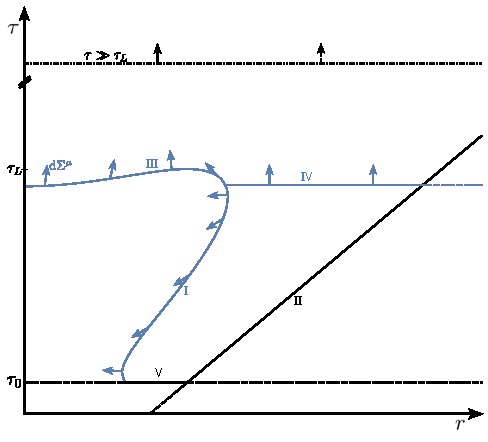
\includegraphics[width=0.4\linewidth]{images/FreezeOutSurface.pdf}
        \captionof{figure}{Freezeout surface in $\tau$-$r$-plane\cite{KirchnerEtAl_2023}.}
        \label{fig:FreezeOutSurface_rtau}
    \end{minipage}
}
Consider the freezeout on the hypersurface depicted in \ref{fig:FreezeOutSurface_rtau}. Assume that the condensate contribution as a function in phase space $f_{\text{cond}}(x^\mu,\vec{p})$ vanishes on $\Sigma_{\text{\rom{2}}}$ and $\Sigma_{\text{\rom{5}}}$, i.e. is contained within the union of all light cones starting on the freeze out surface $\Sigma_{FO}\equiv\Sigma_{\text{\rom{1}}}\cap\Sigma_\text{{\rom{3}}}$. \todo{By causality this seems reasonable, but from Fourier decomposition of a classical field this is not at all clear.} Following the reasoning from \cite{KirchnerEtAl_2023}, we wish to apply Gauß law. Consider separately the contribution on the $\tau$-axis
\begin{equation*}
    \int_{\Sigma_{r=0}}\dt\Sigma^\mu\,J_\mu\qquad\text{or}\qquad\lim_{r\to 0}\int_{\Sigma_{r}}\dt\Sigma^\mu\,J_\mu
\end{equation*}
The surface vector on this hypersurface is $\dt\Sigma_\mu=r\tau\dt\tau\dt\eta\dt\varphi(0,1,0,0)$ and thus vanishes at $r=0$ (the hypersurface $\Sigma_{r=0}$ has zero $3$-volume). Since the derivative of a rotationally symmetric integrand introduces no divergencies, the contribution of $\Sigma_{r=0}$ to Gauß law is zero.
\begin{equation}
    (\phi_J,u_{\vec{p}}^{(*)})_{\Sigma_t}=(\phi,u_{\vec{p}}^{(*)})_{\Sigma_{\tau\gg\tau_L}}=(\phi,u_{\vec{p}}^{(*)})_{\Sigma_{FO}}
\end{equation}

\subsection{Coordinates on the Freezeout Surface}

The freezeout hypersurface is parametrized as $\Sigma_{\text{FO}}=\{x^\mu\in\mathbb{R}^{(1,3)}\vert (\tau,r)=(\tau(\alpha),r(\alpha))\}$ with $\tau,r$ defined by the coordinate transformation
\begin{equation}
    \left\{\begin{split}
        t&=\tau\cosh\eta\\
        z&=\tau\sinh\eta\\
        x&=r\cos\varphi\\
        y&=r\sin\varphi
    \end{split}\right.
    \qquad\iff\qquad
    \left\{\begin{split}
        \tau&=\sqrt{t^2-z^2}\\
        \eta&=\artanh(z/t)\\
        r&=\sqrt{x^2+y^2}\\
        \varphi&=\arctan(y/x)
    \end{split}\right.
\end{equation}

\begin{calc}[Metric on Hypersurface]{calc:HypersurfaceMetric}
    Recall the metric $g_{\mu\nu}=\text{diag}(-1,1,\tau^2,r^2)$ in coordinates $(\tau,r,\eta,\varphi)$. Orthonormal tangent vectors to the freeze out hypersurface are $(\hat\partial_\varphi)^\mu=(0,0,0,r^{-1})=r^{-1}(\partial_\varphi)^\mu$, $(\hat\partial_\eta)^\mu=(0,0,\tau^{-1},0)=\tau^{-1}(\partial_\eta)^\mu$ and $(\hat\partial_\alpha)^\mu=\sqrt{r^{\prime 2}(\alpha)-\tau^{\prime 2}(\alpha)}^{-1}(\tau^{\prime}(\alpha),r^{\prime}(\alpha),0,0)=D(\alpha)(\partial_\alpha)^\mu$ with $D(\alpha)=\sqrt{r^{\prime 2}(\alpha)-\tau^{\prime 2}(\alpha)}^{-1}$. The projector on the hypersurface is
    \begin{equation}
        \gamma_{\mu\nu}=(\hat\partial_\varphi)_\mu(\hat\partial_\varphi)_\nu+(\hat\partial_\eta)_\mu(\hat\partial_\eta)_\nu+(\hat\partial_\alpha)_\mu(\hat\partial_\alpha)_\nu=\begin{pmatrix}
            D^2(\alpha)\tau^{\prime2}(\alpha)               & -D^2(\alpha)\tau^\prime(\alpha)r^\prime(\alpha) & 0      & 0   \\
            -D^2(\alpha)\tau^\prime(\alpha)r^\prime(\alpha) & D^2(\alpha)r^{\prime2}(\alpha)                  & 0      & 0   \\
            0                                               & 0                                               & \tau^2 & 0   \\
            0                                               & 0                                               & 0      & r^2
        \end{pmatrix}
    \end{equation}
    The normal of the hypersurface is $n^\mu\equiv(\hat\partial_\alpha^\perp)^\mu=D(\alpha)(r^\prime(\alpha),\tau^\prime(\alpha),0,0)$ and is timelike where $D$ is real. Naturally $\gamma_{\mu\nu}n^\nu=0$. In the basis $(\partial_\alpha,\partial_\eta,\partial_\varphi,n)$ using (in short form)
    \begin{equation}
        (\partial_\alpha)^\nu\gamma_{\mu\nu}(\partial_\alpha)^\mu=\begin{pmatrix}
            \tau^\prime \\r^\prime
        \end{pmatrix}^T\begin{pmatrix}
            -\tau^\prime \\
            r^\prime
        \end{pmatrix}=D^{-2}
    \end{equation}
    the hypersurface metric in coordinates $x^i=(\alpha,\eta,\varphi)$ reads
    \begin{equation}
        \gamma_{ij}=\text{diag}(D^{-2}(\alpha),\tau^2(\alpha),r^2(\alpha))
    \end{equation}
    and the volume element is given by $\dt\Sigma=r(\alpha)\tau(\alpha) D^{-1}(\alpha)\dt\alpha\dt\eta\dt\varphi$. The oriented surface element is \begin{equation}
        \dt\Sigma^\mu=n^\mu\dt\Sigma=r(\alpha)\tau(\alpha)(r^\prime(\alpha),\tau^\prime(\alpha),0,0)\dt\alpha\dt\eta\dt\varphi
    \end{equation}
\end{calc}

It is also useful to evaluate $p_\mu x^\mu$ in the Bjorken coordinate system. Therefore introduce an analogous coordinate change in momentum space
\begin{equation}
    \left\{\begin{split}
        p_t&=m_\perp\cosh\eta_p\\
        p_z&=m_\perp\sinh\eta_p\\
        p_x&=p_\perp\cos\varphi_p\\
        p_y&=p_\perp\sin\varphi_p
    \end{split}\right.
\end{equation}
to rewrite the scalar product as
\begin{equation}
    p_\mu x^\mu\equiv-\tau(p_t\cosh\eta-p_z\sinh\eta)+r(p_x\cos\varphi+p_y\sin\varphi)=-\tau m_\perp\cosh(\eta-\eta_p)+r p_\perp\cos(\varphi-\varphi_p)
\end{equation}
We used the identities
\begin{equation}
    \cosh(a-b)=\cosh a\cosh b-\sinh a\sinh b\,,\qquad\cos(a-b)=\cos a\cos b+\sin a\sin b
\end{equation}
The integral measure changes according to $\dt^4p_{\text{cart}}=\dt m_\perp\dt p_\perp\dt\eta_p\dt\varphi_p\cdot m_\perp p_\perp$. The momentum shell condition $p^2+m^2=0$ is equivalently parametrized by $m_\perp^2=p_\perp^2+m^2\eqdef \omega_\perp^2$.

\subsection{Converting Spectra between Coordinate Systems}
\label{sec:SpectraCoordinateSystem}

Consider the coordinate change in momentum space
\begin{equation}
    \left\{
    \begin{split}
        p_x&=p^\perp\cos\varphi_p\\
        p_y&=p^\perp\sin\varphi_p\\
        p_z&=m^\perp\sinh\eta_p\\
        p_t&=m^\perp\cosh\eta_p
    \end{split}
    \right.\qquad\iff\qquad
    \left\{
    \begin{split}
        p^\perp&=\sqrt{p_x^2+p_y^2}\\
        \varphi_p&=\arctan(p_y/p_y)\\
        m^\perp&=\sqrt{p_t^2-p_z^2}\\
        \eta_p&=\artanh(p_z/p_t)
    \end{split}
    \right.
\end{equation}
with Jacobian
\begin{equation}
    \big\vert\frac{\partial(p^\perp,\varphi_p,m^\perp,\eta_p)}{\partial(p_x,p_y,p_z,p_t)}\big\vert=\frac{1}{m^\perp p^\perp}
\end{equation}
Let $f(p_\mu)$ be some distribution function and $F$ its momentum space integral evaluated on the momentum shell and future directed momenta.

\begin{subequations}
    \begin{align}
        F=\int\frac{\dt^4p_{\text{cart}}}{(2\pi)^4}\delta(p^2+m^2)\Theta(p_t)f(p_\mu) & =\int\frac{\dt p_t}{2\pi}\int\frac{\dt^3p_{\text{cart}}}{(2\pi)^3}\frac{1}{2\omega_{\vec{p}}}\big(\delta(p_t-\omega_{\vec{p}})+\delta(p_t+\omega_{\vec{p}})\big)\Theta(p_t)f(p_\mu) \\
                                                                                      & =\frac{1}{2\pi}\int\frac{\dt^3p_{\text{cart}}}{(2\pi)^3}\frac{1}{2\omega_{\vec{p}}}f(p_\mu)\big\vert_{p_t=\omega_{\vec{p}}}
    \end{align}
    On the other hand
    \begin{align}
        F=\int\frac{\dt^4p_{\text{cart}}}{(2\pi)^4}\delta(p^2+m^2)\Theta(p_t)f(p_\mu) & =\frac{1}{(2\pi)^4}\int_0^\infty \dt p^\perp\int_0^\infty \dt m^\perp\int_{-\infty}^\infty \dt\eta_p\int_0^{2\pi}\dt\varphi_pm^\perp p^\perp\times\nonumber \\
                                                                                      & \phantom{=}\qquad\times\delta((p^\perp)^2-(m^\perp)^2+m^2)f(p_\mu)                                                                                              \\
        \intertext{assume $f(p^\mu)=f(p^\perp,m^\perp,\eta_p)$ and perform the $\varphi$-integraion as well as $m^\perp$-integration, where $\omega^{\perp,2}=m^2+p^{\perp,2}$ is defined}
                                                                                      & =\frac{1}{(2\pi)^3}\int_0^\infty\dt p^\perp\int_{-\infty}^\infty\dt\eta_p\frac{p^\perp}{2}f(p_\mu)\big\vert_{m^\perp=\omega^\perp}
    \end{align}
    leding to the important result
    \begin{equation}
        \frac{1}{2\pi}\int\frac{\dt^3p_{\text{cart}}}{(2\pi)^3}\frac{1}{2\omega_{\vec{p}}}f(p_\mu)\big\vert_{p_t=\omega_{\vec{p}}}=\frac{1}{(2\pi)^3}\int_0^\infty\dt p^\perp\int_{-\infty}^\infty\dt\eta_p\frac{p^\perp}{2}f(p_\mu)\big\vert_{m^\perp=\omega^\perp}
    \end{equation}
\end{subequations}

Since the restrictions $p_t=\omega_{\vec{p}}$ and $m^\perp=\omega^\perp$ are equivalent (considering the parametrization that already satisfies $p_t=p^\perp\cosh\eta_p\geq 0$) we find
\begin{equation}
    \omega_{\vec{p}}\frac{\dt F}{\dt p_x\dt p_y\dt p_z}=\frac{1}{2\pi p^\perp}\frac{\dt F}{\dt p^\perp\dt\eta_p}
\end{equation}
The result applies to the case
\begin{equation}
    f(p_\mu)\big\vert_{p_t=\omega_{\vec{p}}}=2\omega_{\vec{p}}\cdot 2\pi\cdot n(\vec{p})
\end{equation}
and $F=N$. \textbf{\textcolor{red}{This holds for the symmetric range $\eta\in(-\infty,\infty)$. Restricting to $\eta\in[0,\infty)$ we find
\begin{equation}
    2\omega_{\vec{p}}\frac{\dt F}{\dt p_x\dt p_y\dt p_z}=\frac{1}{2\pi p^\perp}\frac{\dt F}{\dt p^\perp\dt\eta_p}
\end{equation}
}}

\subsection{Computing the Inner Product}

The projection of the derivative onto the surface normal of $\Sigma_{\text{FO}}$  is (omitting the $\alpha$-dependence) 
\begin{equation}
    \dt\Sigma^\mu\partial_\mu=(r^\prime\partial_\tau+\tau^\prime\partial_r)\cdot r\tau\,\dt\alpha\dt\eta\dt\varphi
\end{equation}
For the real scalar field $\pi^0$, following the ideas of section \ref{sec:FluidFromRealScalar}, one finds
\begin{equation}
    \dt\Sigma^\mu\partial_\mu=\chi(r^\prime \underbrace{u_\tau}_{\textcolor{red}{=-u^\tau}}+\tau^\prime u_r)\cdot r\tau\,\dt\alpha\dt\eta\dt\varphi
\end{equation}

It is useful to compute the following integrals related to Bessel functions: \url{https://dlmf.nist.gov/10.9}
\begin{subequations}
    \begin{align}
        \int_0^{2\pi}\dt\varphi e^{\pm\imagu a\cos\varphi}&=\int_0^{2\pi}\big(\cos(a\cos\varphi)\pm\imagu\sin(a\cos\varphi)\big)=2\int_0^\pi\cos(a\cos\varphi)\\
        &=2\pi J_0(a)\\
        \int_{-\infty}^\infty\dt\eta e^{\pm\imagu a\cosh\eta}&=2\int_0^\infty\dt\eta\big(\cos(a\cosh\eta)\pm\imagu\sin(a\cosh\eta)\big)\\
        &=\pi\big(-Y_0(a)\pm\imagu J_0(a)\big)\\
        &=\pm\pi\imagu(J_0(a)\pm\imagu Y_0(a))=\begin{cases}
            +\pi\imagu H^{(1)}_0(a)&\text{for "+"}\\
            -\pi\imagu H^{(2)}_0(a)&\text{for "-"}
        \end{cases}
    \end{align}
    Additionally to the integral representations, the following computation makes use of \url{https://dlmf.nist.gov/10.4}
    \begin{equation}
        J_{0}^\prime(x)=-J_1(x)\,,\qquad Y_0^\prime(x)=-Y_1(x)
    \end{equation}
\end{subequations}

\begin{subequations}
    \begin{align}
        J(\pm p) & =-\int_{-\infty}^\infty\dt\eta\int_0^{2\pi}\dt\varphi\int_0^\pi\dt\alpha\tau r\Bigg[\phi(\tau,r)\big(r^\prime\overset{\leftrightarrow}{\partial_\tau}+\tau^\prime\overset{\leftrightarrow}{\partial_r}\big)e^{\pm\imagu(\tau \omega_\perp\cosh(\eta-\eta_p)-r p_\perp\cos(\varphi-\varphi_p))}\Bigg] \\
                           & =-\int_{-\infty}^\infty\dt\eta\int_0^{2\pi}\dt\varphi\int_0^\pi\dt\alpha\tau r\Bigg[\phi(\tau,r)\big(r^\prime\overset{\leftrightarrow}{\partial_\tau}+\tau^\prime\overset{\leftrightarrow}{\partial_r}\big)e^{\pm\imagu(\tau \omega_\perp\cosh\eta-r p_\perp\cos\varphi)}\Bigg]                      \\
                           & =-2\pi^2\int_0^\pi\dt\alpha\tau r\Bigg[\phi(\tau,r)(r^\prime\overset{\leftrightarrow}{\partial_\tau}+\tau^\prime\overset{\leftrightarrow}{\partial_r})\Big[J_0(r p_\perp)\times\big(-Y_0(\tau\omega_\perp)\pm\imagu J_0(\tau\omega_\perp)\big)\Big]\Bigg]                                                 \\
                           & =2\pi^2\int_0^\pi\dt\alpha\tau r\Bigg[(r^\prime\partial_\tau+\tau^\prime\partial_r)\phi(\tau,r)\Big[J_0(r p_\perp)\times\big(-Y_0(\tau\omega_\perp)\pm\imagu J_0(\tau\omega_\perp)\big)\Big]+\nonumber                                                                                             \\
                           & \phantom{=}\qquad + \phi(\tau,r)\Big[\tau^\prime\times p_\perp J_1(r p_\perp)\times\big(-Y_0(\tau\omega_\perp)\pm\imagu J_0(\tau\omega_\perp)\big)+\nonumber                                                                                                                                       \\
                           & \phantom{=}\qquad\phantom{+\phi(\tau,r)\Big[}+r^\prime\times J_0(r p_\perp)\times\omega_\perp\big(-Y_1(\tau\omega_\perp)\pm\imagu J_1(\tau\omega_\perp)\big)\Big]\Bigg]
    \end{align}
\end{subequations}

\begin{subequations}
    \begin{align}
        J(\overset{(-)}{+}p) & =-\int_{-\infty}^\infty\dt\eta\int_0^{2\pi}\dt\varphi\int_0^\pi\dt\alpha\tau r\Bigg[\phi(\tau,r)\big(r^\prime\overset{\leftrightarrow}{\partial_\tau}+\tau^\prime\overset{\leftrightarrow}{\partial_r}\big)e^{\overset{(-)}{+}\imagu(\tau \omega_\perp\cosh(\eta-\eta_p)-r p_\perp\cos(\varphi-\varphi_p))}\Bigg] \\
                           & =-\int_{-\infty}^\infty\dt\eta\int_0^{2\pi}\dt\varphi\int_0^\pi\dt\alpha\tau r\Bigg[\phi(\tau,r)\big(r^\prime\overset{\leftrightarrow}{\partial_\tau}+\tau^\prime\overset{\leftrightarrow}{\partial_r}\big)e^{\overset{(-)}{+}\imagu(\tau \omega_\perp\cosh\eta-r p_\perp\cos\varphi)}\Bigg]                      \\
                           & =\overset{(+)}{-}2\pi^2\imagu\int_0^\pi\dt\alpha\tau r\Bigg[\phi(\tau,r)(r^\prime\overset{\leftrightarrow}{\partial_\tau}+\tau^\prime\overset{\leftrightarrow}{\partial_r})\Big[J_0(r p_\perp)\times H_0^{\overset{(2)}{(1)}}(\tau\omega_\perp)\Big]\Bigg]                                                 \\
                           & =\overset{(-)}{+}2\pi^2\imagu\int_0^\pi\dt\alpha\tau r\Bigg[(r^\prime\partial_\tau+\tau^\prime\partial_r)\phi(\tau,r)\Big[J_0(r p_\perp)\times H_0^{\overset{(2)}{(1)}}(\tau\omega_\perp)\Big]+\nonumber                                                                                             \\
                           & \phantom{=}\qquad + \phi(\tau,r)\Big[\tau^\prime\times p_\perp J_1(r p_\perp)\times H_0^{\overset{(2)}{(1)}}(\tau\omega_\perp)+r^\prime\times J_0(r p_\perp)\times\omega_\perp H_1^{\overset{(2)}{(1)}}(\tau\omega_\perp)\Big]\Bigg]
    \end{align}
\end{subequations}

\section{Considering Resonance Decays}

If the particles considered on the freezout surface are not stable, the spectra computed there cannot be directly related to the spectra on the detector surface. Instead, one has to calculate contributions from all possible decay channels/heavier resonances $a$ that decay into the (stable) resonance $b$ under consideration. This is done via the linear decay map
\begin{equation}
    E_{\vec{p}}\frac{\dt N_b}{\dt^3p}=\int\frac{\dt^3q}{(2\pi)^3}\frac{1}{2\omega_{\vec{p}}}D_{a\rightarrow b}(\vec{p},\vec{q})E_{\vec{q}}\frac{\dt N_a}{\dt^3 q}
\end{equation} 
where $D_{a\rightarrow b}(\vec{p},\vec{q})$ is the Lorentz invariant probability of particle $a$ with (on-shell) momentum $\vec{q}$ to decay into particle $b$ with momentum $\vec{p}$. Due to the probabilistic nature of a decay process, this relation is true if the lifetime of the heavy resonances is short compared to the propagation time and the number of particles is large enough.

Assuming isotropic decay, a two-body decay $a\rightarrow b+c$ is modelled by the decay map 
\begin{equation}
    D_{a\rightarrow b\vert c}(\vec{p},\vec{q})=D_{a\rightarrow b\vert c}(p^\mu q_\mu)=B\frac{4\pi^2 m_a}{p_{a\rightarrow b\vert c}}\delta(q^\mu p_\mu+m_a E_{a\rightarrow b\vert c})
\end{equation}
where $B$ is the branching ratio of the decay and
\begin{equation}
    p_{a\rightarrow b\vert c}=\frac{1}{2m_a}\sqrt{\big((m_a+m_b)^2-m_c^2\big)\big((m_a-m_b)^2-m_c^2\big)}\,,\qquad E_{a\rightarrow b\vert c}=\sqrt{m_b^2+p_{a\rightarrow b\vert c}^2}
\end{equation}
In the rest frame of particle $a$ one finds $\vec{p}\equiv \vec{p}_b=-\vec{p}_c$, energy conservation is expressed as
\begin{equation}
    m_a=\sqrt{m_b^2+\vec{p}^2}+\sqrt{m_c^2+\vec{p}^2}
\end{equation}
with the solution space restricted only by $\vec{p}^2=p_{a\rightarrow b\vert c}^2$. The energy of particle $b$ in the rest frame of $a$, expressed covariantly, is just $E_{a\rightarrow b\vert c}=-\frac{1}{m_a}q^\mu p_\mu$ and thus the above formula simply represents energy conservation.

To decompose the above delta function, rewrite $q^\mu p_\mu$ in the coordinates used in \ref{sec:SpectraCoordinateSystem}.
\begin{equation}
    q^\mu p_\mu=-m_q^\perp m_p^\perp\cosh(\eta_q-\eta_p)+q^\perp p^\perp\cos(\varphi_q-\varphi_p)
\end{equation}
Later we shall resolve the $\delta$-distribution using the identity
\begin{equation}
    \int\dt^dx f(x^i)\delta(g(x^i))=\int_{g^{-1}(0)}\dt^{d-1}\sigma\frac{f(x^i)}{\Vert\vec{\nabla}g(x^i)\Vert}
\end{equation}
    
\begin{subequations}
    \begin{align}
        \omega_{\vec{p}}\frac{\dt N_b}{\dt^3p}&=B\frac{4\pi^2m_a}{p_{a\rightarrow b\vert c}}\times2\pi\int\frac{\dt^4q}{(2\pi)^4}\delta(q^2+m^2)\Big(\omega_{\vec{q}}\frac{\dt N_a}{\dt^3 q}\Big)\delta\big(q^\mu p_\mu+m_a E_{a\rightarrow b\vert c}\big)\\
        &=B\frac{4\pi^2m_a}{p_{a\rightarrow b\vert c}}\times2\pi\int_{(0,0,-\infty,0)}^{(\infty,\infty,\infty,2\pi)}\frac{\dt m_q^\perp \dt q^\perp\dt\eta_q\dt\varphi_q}{(2\pi)^4}m_q^\perp q^\perp\delta(-m_q^{\perp,2}+q^{\perp,2}+m^2)\Big(\omega_{\vec{q}}\frac{\dt N_a}{\dt^3 q}\Big)\times\nonumber\\
        &\phantom{=}\qquad\times\delta\big(-m_q^\perp m_p^\perp\cosh(\eta_q-\eta_p)+q^\perp p^\perp\cos(\varphi_q-\varphi_p)+m_a E_{a\rightarrow b\vert c}\big)\\
        % &=B\frac{4\pi^2m_a}{p_{a\rightarrow b\vert c}}\times2\pi\int_{(0,-\infty,0)}^{(\infty,\infty,2\pi)}\frac{\dt q^\perp\dt\eta_q\dt\varphi_q}{(2\pi)^4}\frac{q^\perp}{2}\omega_{\vec{q}}\frac{\dt N_a}{\dt^3 q}\times\nonumber\\
        % &\phantom{=}\qquad\times\delta\big(-\omega_q^\perp \omega_p^\perp\cosh(\eta_q-\eta_p)+q^\perp p^\perp\cos(\varphi_q-\varphi_p)+m_a E_{a\rightarrow b\vert c}\big)\\
        &=B\frac{4\pi^2m_a}{p_{a\rightarrow b\vert c}}\times2\pi\int_{(0,-\infty,0)}^{(\infty,\infty,2\pi)}\frac{\dt q^\perp\dt\eta_q\dt\varphi_q}{(2\pi)^4}\frac{q^\perp}{2}\Big(\omega_{\vec{q}}\frac{\dt N_a}{\dt^3 q}\Big)\times\nonumber\\
        &\phantom{=}\qquad\times\delta\big(-\omega_q^\perp \omega_p^\perp\cosh\eta_q+q^\perp p^\perp\cos\varphi_q+m_a E_{a\rightarrow b\vert c}\big)\\
        &=B\frac{4\pi^2m_a}{p_{a\rightarrow b\vert c}}\times2\pi\times 2\times 2\int_{(0,0,0)}^{(\infty,\infty,\pi)}\frac{\dt q^\perp\dt\eta_q\dt\varphi_q}{(2\pi)^4}\frac{q^\perp}{2}\Big(\omega_{\vec{q}}\frac{\dt N_a}{\dt^3 q}\Big)\times\nonumber\\
        &\phantom{=}\qquad\times\delta\big(-\omega_q^\perp \omega_p^\perp\cosh\eta_q+q^\perp p^\perp\cos\varphi_q+m_a E_{a\rightarrow b\vert c}\big)\\
        &=B\frac{4\pi^2m_a}{p_{a\rightarrow b\vert c}}\times2\pi\times 2\times 2\times(q^\perp)^2\times\int_{(0,1,-1)}^{(\infty,\infty,1)}\frac{\dt t\dt u\dt v}{(2\pi)^4}\frac{t}{2}\Big(\omega_{\vec{q}}\frac{\dt N_a}{\dt^3 q}\Big)\frac{1}{\sqrt{u^2-1}}\frac{1}{\sqrt{1-v^2}}\times\nonumber\\
        &\phantom{=}\qquad\times\delta\big(-\omega_q^\perp \omega_p^\perp u+q^\perp p^\perp tv+m_a E_{a\rightarrow b\vert c}\big)\\
        &=B\frac{4\pi^2m_a}{p_{a\rightarrow b\vert c}}\times\frac{4\pi(\tilde{q}^\perp)^2}{(2\pi)^4}\times\int_0^\infty\dt t\int_{-1}^1\dt v\;t\;\Big(\omega_{\vec{q}}\frac{\dt N_a}{\dt^3 q}\Big)\Big\vert_{t\cdot \tilde{q}^\perp }\Bigg(\frac{\Theta(u-1)}{\sqrt{u^2-1}}\frac{1}{\sqrt{1-v^2}}\frac{\sigma(t,v)}{\Vert\vec{\nabla}g(t,u,v)\Vert}\Bigg)\Bigg\vert_{u=u^\star(t,v)}        
    \end{align}
\end{subequations}
\vspace{3em}
\begin{equation}
    \eqnmarkbox[blue]{myeq}{\omega_{\vec{p}}\frac{\dt N_b}{\dt^3p}=\frac{B(\tilde{q}^\perp)^2}{p_{a\rightarrow b\vert c}\pi}\int_0^\infty\dt t\int_{-1}^1\dt v\;t\;\Big(\omega_{\vec{q}}\frac{\dt N_a}{\dt^3 q}\Big)\Big\vert_{t\cdot \tilde{q}^\perp }\Bigg(\frac{\Theta(u-1)}{\sqrt{u^2-1}}\frac{1}{\sqrt{1-v^2}}\frac{\sigma(t,v)}{\Vert\vec{\nabla}g(t,u,v)\Vert}\Bigg)\Bigg\vert_{u=u^\star(t,v)}}
\end{equation}
where we made use of rotational and boost symmetry to eliminate the $\varphi_p$ and $\eta_p$ dependence and applied the variable changes
\begin{gather*}
    \int_0^\infty\dt\eta\;f(\cosh\eta)=\int_1^\infty\dt u\frac{f(u)}{\sqrt{u^2-1}}\,,\qquad \int_0^\pi\dt\varphi\;f(\cos\varphi)=\int_{-1}^1\dt v\frac{f(v)}{\sqrt{1-v^2}}\\
   \text{and}\qquad q^\perp=\tilde{q}^\perp t\quad\text{with}\;\tilde{q}^\perp=\const\;\text{and}\;[\tilde{q}^\perp]=\text{GeV}\,,\;[t]=1
\end{gather*}
(omit the $\tilde{\cdot}$ in the following) and defined $u^\star(t,v)$ to respect the $\delta$. The $\delta$-distribution depending on the variables $(t,u,v)$ and the parameters $(q^\perp,p^\perp)$ was replaced by considering the function
\begin{subequations}
    \begin{align}
        g(t,u,v)&=-\omega_q^\perp \omega_p^\perp u+q^\perp p^\perp tv+m_a E_{a\rightarrow b\vert c}\\
        \vec{\nabla} g&=
        \begin{pmatrix}
            -t\,u\,\frac{\omega_p^\perp}{\omega_q^\perp}(q^\perp)^2+q^\perp p^\perp v\\
            -\omega_q^\perp\omega_p^\perp\\
            t\,q^\perp p^\perp
        \end{pmatrix}
    \end{align}
\end{subequations}
The manifold defined by the level set where $g(t,u,v)=0$ is given by 
\begin{equation}
    g^{-1}(0)=\Bigg\{(t,u,v)\Big\vert u=u^\star(t,v)=\frac{m_aE_{a\rightarrow b\vert c}+q^\perp p^\perp tv}{\omega_q^\perp\omega_p^\perp}\Bigg\}
    \label{eq:DecayMap_BjorkenCoord_DeltaManifold}
\end{equation}
\eqref{eq:DecayMap_BjorkenCoord_DeltaManifold} defines a chart $(t,v)\mapsto x^i(t,v)=(t,u^\star(t,v),v)$ on $g^{-1}(0)$ with coordinates $(t,v)$. One computes the coordinate derivative vectors and oriented surface element
\begin{equation}
    \frac{\partial x^i}{\partial t}=\begin{pmatrix}
    1\\
    v\frac{p^\perp q^\perp}{\omega_p^\perp\omega_q^\perp}\big(1-t^2\frac{(q^\perp)^2}{(\omega_q^\perp)^2}\big)\\
    0
    \end{pmatrix}\,,\quad
    \frac{\partial x^i}{\partial v}=\begin{pmatrix}
        0\\
        t\frac{q^\perp p^\perp}{\omega_q^\perp\omega_p^\perp}\\
        1
    \end{pmatrix}\,,\quad
    \dt\Sigma^i=\frac{\partial x^i}{\partial q^\perp}\times \frac{\partial x^i}{\partial q^\perp}\dt t\dt v=\begin{pmatrix}
        v\frac{p^\perp q^\perp}{\omega_p^\perp\omega_q^\perp}\big(1-t^2\frac{(q^\perp)^2}{(\omega_q^\perp)^2}\big)\\
        -1\\
        t\frac{q^\perp p^\perp}{\omega_q^\perp\omega_p^\perp}
    \end{pmatrix}\dt t\dt v
\end{equation}
which defines the scalar surface element via $\dt^2\sigma=\sigma(t,v)\dt t\dt v=\Vert\dt\Sigma^i\Vert$.

Investigate the large $t$ behaviour of $u^\star(t,v)$. The claim is that there is always a $t_{\text{max}}(v,p^\perp)$ such that $u^*(t>t_{\text{max}},v)<1$. Since $u^*(t,1)\geq u^*(t,v\in[-1,1])$ it suffices to consider the case $v=1$. Also note that $\frac{p^\perp}{\omega_p^\perp}<1$ for every finite $p^\perp$. Since analogously $\lim_{t\to\infty}\frac{q^\perp t}{\omega_q^\perp}=1$ and the "$+m_aE_{a\rightarrow b\vert c}$" becomes irrelevant in the limit, one arrives at $\lim_{t\to\infty}u^\star(t,v)<1$.

% \paragraph*{Again without Change of Variables}\mbox{}\\

% \begin{subequations}
%     \begin{align}
%         \omega_{\vec{p}}\frac{\dt N_b}{\dt^3p}&=B\frac{4\pi^2m_a}{p_{a\rightarrow b\vert c}}\times2\pi\int\frac{\dt^4q}{(2\pi)^4}\delta(q^2+m^2)\omega_{\vec{q}}\frac{\dt N_a}{\dt^3 q}\delta\big(q^\mu p_\mu+m_a E_{a\rightarrow b\vert c}\big)\\
%         &=B\frac{4\pi^2m_a}{p_{a\rightarrow b\vert c}}\times2\pi\int_{(0,0,-\infty,0)}^{(\infty,\infty,\infty,2\pi)}\frac{\dt m_q^\perp \dt q^\perp\dt\eta_q\dt\varphi_q}{(2\pi)^4}m_q^\perp q^\perp\delta(-m_q^{\perp,2}+q^{\perp,2}+m^2)\omega_{\vec{q}}\frac{\dt N_a}{\dt^3 q}\times\nonumber\\
%         &\phantom{=}\qquad\times\delta\big(-m_q^\perp m_p^\perp\cosh(\eta_q-\eta_p)+q^\perp p^\perp\cos(\varphi_q-\varphi_p)+m_a E_{a\rightarrow b\vert c}\big)\\
%         &=B\frac{4\pi^2m_a}{p_{a\rightarrow b\vert c}}\times2\pi\int_{(0,-\infty,0)}^{(\infty,\infty,2\pi)}\frac{\dt q^\perp\dt\eta_q\dt\varphi_q}{(2\pi)^4}\frac{q^\perp}{2}\omega_{\vec{q}}\frac{\dt N_a}{\dt^3 q}\times\nonumber\\
%         &\phantom{=}\qquad\times\delta\big(-\omega_q^\perp \omega_p^\perp\cosh\eta_q+q^\perp p^\perp\cos\varphi_q+m_a E_{a\rightarrow b\vert c}\big)\\
%         &=B\frac{4\pi^2m_a}{p_{a\rightarrow b\vert c}}\times2\pi\times 2\times 2\int_{(0,0,0)}^{(\infty,\infty,\pi)}\frac{\dt q^\perp\dt\eta_q\dt\varphi_q}{(2\pi)^4}\frac{q^\perp}{2}\omega_{\vec{q}}\frac{\dt N_a}{\dt^3 q}\times\nonumber\\
%         &\phantom{=}\qquad\times\delta\big(-\omega_q^\perp \omega_p^\perp\cosh\eta_q+q^\perp p^\perp\cos\varphi_q+m_a E_{a\rightarrow b\vert c}\big)\\
%         \intertext{\dots using $q^\perp\mapsto t\cdot \tilde{q}^\perp$, where $\tilde{q}^\perp=\const$ carries the dimension and $t\in[0,\infty)$ is dimensionless, we calculate (omit the $\tilde{\cdot}$)}
%         &=B\frac{4\pi^2m_a}{p_{a\rightarrow b\vert c}}\times\frac{4\pi(q^\perp)^2}{(2\pi)^4}\times\int_0^\infty\dt t\int_0^\pi\dt\varphi\cdot t\cdot \Big(\omega_{\vec{q}}\frac{\dt N_a}{\dt^3 q}\Big)\Big\vert_{t\cdot q^\perp}\frac{\sigma(t,\varphi)}{\Vert\vec{\nabla}g(t,\eta^\star,\varphi)\Vert}
%     \end{align}
% \end{subequations}
% Here we defined
% \begin{subequations}
%     \begin{align}
%         g(t,\eta,\varphi)&=-\omega_q^\perp \omega_p^\perp \cosh\eta+q^\perp p^\perp t\cos\varphi+m_a E_{a\rightarrow b\vert c}\\
%         \vec{\nabla} g&=
%         \begin{pmatrix}
%             -\frac{\omega_p^\perp}{\omega_q^\perp}(q^\perp)^2 \cdot t\cdot\cosh\eta+q^\perp p^\perp \cos\varphi\\
%             -\omega_q^\perp\omega_p^\perp\sinh\eta\\
%             -t\cdot q^\perp p^\perp\sin\varphi
%         \end{pmatrix}
%     \end{align}
% \end{subequations}
% implying 
% \begin{equation}
%     g^{-1}(0)=\Bigg\{(t,\eta,\varphi)\Big\vert\eta=\eta^\star(t,\varphi)=\arcosh\Big(\underbrace{\frac{m_a E_{a\rightarrow b\vert c}+t\cdot q^\perp p^\perp\cos\varphi}{\omega_q^\perp\omega_p^\perp}}_{\eqdef u^\star(t,\varphi)}\Big)\Bigg\}
% \end{equation}
% One this manifold we need the surface element $\sigma(t,\varphi)\dt t\dt\varphi$. For some $x^i\in g^{-1}(0)$ the coordinate derivatives and surface normal are given by
% \begin{subequations}
%     \begin{align}        
%         \frac{\partial x^i}{\partial t}=\begin{pmatrix}
%             1\\
%             \frac{1}{\sqrt{(u^\star)^2-1}}\frac{\partial u^\star}{\partial t}\\
%             0
%         \end{pmatrix}&=\begin{pmatrix}
%             1\\
%         \frac{1}{\sqrt{(u^\star)^2-1}}\cdot\frac{q^\perp p^\perp}{\omega_q^\perp\omega_p^\perp}\cos\varphi\Big(1-t^2\big(\frac{q^\perp}{\omega_q^\perp}\big)^2\Big)\\
%         0
%     \end{pmatrix}\\
%     \frac{\partial x^i}{\partial \varphi}=\begin{pmatrix}
%         0\\
%         \frac{1}{\sqrt{(u^\star)^2-1}}\frac{\partial u^\star}{\partial\varphi}\\
%         1
%     \end{pmatrix}&=\begin{pmatrix}
%         0\\
%         -\frac{1}{\sqrt{(u^\star)^2-1}}\frac{q^\perp p^\perp}{\omega_q^\perp\omega_p^\perp}\cdot t\sin\varphi\\
%         1
%     \end{pmatrix}\\
%     \dt^2\sigma^i=\frac{\partial x^i}{\partial t}\times\frac{\partial x^i}{\partial\varphi}\dt t\dt\varphi&=\begin{pmatrix}
%         \frac{1}{\sqrt{(u^\star)^2-1}}\cdot\frac{q^\perp p^\perp}{\omega_q^\perp\omega_p^\perp}\cos\varphi\Big(1-t^2\big(\frac{q^\perp}{\omega_q^\perp}\big)^2\Big)\\
%         -1\\
%         -\frac{1}{\sqrt{(u^\star)^2-1}}\frac{q^\perp p^\perp}{\omega_q^\perp\omega_p^\perp}\cdot t\sin\varphi
%     \end{pmatrix}\dt t\dt\varphi\\
%     \sigma(t,\varphi)\dt t\dt\varphi&\defeq \Vert\dt^2\sigma^i\Vert
% \end{align}
% \end{subequations}

Let us try to evaluate the decay map in the rest frame of the decay product b, such that $p^\mu=(m_b,\vec{0})$.
\begin{subequations}
    \begin{align}
        \omega_{\vec{p}}\frac{\dt N_b}{\dt^3p}&=B\frac{4\pi^2m_a}{p_{a\rightarrow b\vert c}}\times2\pi\int\frac{\dt^4q}{(2\pi)^4}\delta(q^2+m_a^2)\Big(\omega_{\vec{q}}\frac{\dt N_a}{\dt^3 q}\Big)\delta\big(q^\mu p_\mu+m_a E_{a\rightarrow b\vert c}\big)\\
        &=B\frac{4\pi^2m_a}{p_{a\rightarrow b\vert c}}\times2\pi\int\frac{\dt q^0\dt q^3\dt q^\perp q^\perp\dt\varphi}{(2\pi)^4}\delta(q^2+m_a^2)\Big(\omega_{\vec{q}}\frac{\dt N_a}{\dt^3 q}\Big)\delta\big(-m_bq^0+m_a E_{a\rightarrow b\vert c}\big)\\
        &=B\frac{4\pi^2m_a}{p_{a\rightarrow b\vert c}}\times\frac{2\pi}{m_b}\int\frac{\dt q^3\dt q^\perp q^\perp\dt\varphi}{(2\pi)^4}\delta\Big(\underbrace{-\frac{m_a^2E_{a\rightarrow b\vert c}^2}{m_b^2}+m_a^2}_{=-\frac{m_a^2p_{a\rightarrow b\vert c}^2}{m_b^2}}+(q^3)^2+(q^\perp)^2\Big)\Big(\omega_{\vec{q}}\frac{\dt N_a}{\dt^3 q}\Big)\\
        \intertext{\dots define $q^3=w\frac{m_a p_{a\rightarrow b\vert c}}{m_b}$\dots}
        &=B\frac{4\pi^2m_a}{p_{a\rightarrow b\vert c}}\times\frac{(2\pi)^2 m_ap_{a\rightarrow b\vert c}}{m_b^2}\int\frac{\dt w\dt q^\perp q^\perp}{(2\pi)^4}\delta\Big((q^\perp)^2-(1-w^2)\frac{m_a^2p_{a\rightarrow b\vert c}^2}{m_b^2}\Big)\Big(\omega_{\vec{q}}\frac{\dt N_a}{\dt^3 q}\Big)\\
        &=B\frac{4\pi^2m_a}{p_{a\rightarrow b\vert c}}\times\frac{(2\pi)^2 m_ap_{a\rightarrow b\vert c}}{2m_b^2}\int_{-1}^1\frac{\dt w}{(2\pi)^4}\Big(\omega_{\vec{q}}\frac{\dt N_a}{\dt^3 q}\Big)\Big\vert_{q^\perp=q^{\perp,\star}(w)}\\
    \end{align}
\end{subequations}
where we integrated out the $\delta$-function over $q^\perp$, using $\delta((q^\perp)^2-(q^{\perp,\star})^2)=\delta(q^\perp\pm q^{\perp,\star})/(2\vert q^\perp\vert)$ with 
\begin{equation}
    q^{\perp,\star}(w)=\sqrt{(1-w^2)\frac{m_a^2p_{a\rightarrow b\vert c}^2}{m_b^2}}
\end{equation}
and the condition $(q^\perp)^2\geq 0$ implies $w\in[-1,1]$.